% importa variabili globali
% definizione variabili globali
\def\GRUPPO {\textit{DazzleWorks}}

\def\PROGETTO {\textbf{Premi}}

\def\COMMITTENTE {Prof. Vardanega Tullio, \\ & Dr. Cardin Riccardo}

\def\EMAIL {dazzleworksgroup@gmail.com}

\def\LOGO {../../template/img/logo.png}

\def\INTESTAZIONE {../../template/img/intestazione.png}
\def\PIEDIPAGINA {../../template/img/piedipagina.png}

\def\G {{\small $_G$}}


% definizione variabili locali
\def\DOCUMENTO{Analisi dei Requisiti}
\def\VERSIONE{1.0.0}

\def\DESCRIZIONE{Documento che descrive l'analisi dei requisiti e dei casi d'uso del gruppo \GRUPPO per il progetto \PROGETTO}

\def\REDATTORE {Matteo Agostinetto \\ & Nicola Carraro}
\def\VERIFICATORE {<Verificatore>}
\def\RESPONSABILE {Valerio Burlin}

\def\USO {Esterno}

\def\DISTRIBUZIONE {\GRUPPO{}\\ & \COMMITTENTE{}\\}

\def\DESCRIZIONE {Documento che descrive l'analisi dei requisiti e dei casi d'uso del gruppo \GRUPPO per il progetto \PROGETTO}


% abilita (true) / disabilita (false) indice, lista tabelle, lista figure
\def\INDICE	{true}
\def\TABELLE {false}
\def\FIGURE {true}


% importa struttura
\documentclass[a4paper]{article}

% ----- definizioni -----
\def\TITLE		{\mbox{\GRUPPO}}
\def\SUBTITLE	{\SIGLA, \PROGETTO}


% ----- nuovi comandi -----
% fornisce il caption per riferirsi ad una particolare sezione
\newcommand{\numref}[1]{\textsf{\textsl{``\nameref{#1}'' (\ref{#1})}}}


% ----- package -----
\usepackage[T1]{fontenc}   % codifica dei font in uscita
\usepackage[utf8x]{inputenc}   % lettere accentate da tastiera
\usepackage[italian]{babel}   % lingua principale del documento
\usepackage[a4paper, top= 3cm, bottom= 3cm, left= 3cm, right= 3cm, bindingoffset= 5mm]{geometry} % impostazione margini

\usepackage{amssymb} %

\usepackage{booktabs} % comandi aggiuntivi per le tabelle

\usepackage{calc} % espressioni aritmetiche
\usepackage{caption} % descrizione figure, ecc
\usepackage{chapterbib} % inclusione delle bibliografie

\usepackage{datatool} % manipolazione dati
\usepackage{dcolumn} % array in tabular

\usepackage{epstopdf} % conversione eps--> pdf
\usepackage{enumitem} % personalizzazione liste
\usepackage{eurosym} % simbolo euro

\usepackage{fancyhdr}   %personalizzazione dello stile
\usepackage{float} % definizione di oggetti floating (es. figure, tabelle)
\usepackage[bottom]{footmisc} % personalizzazione note

\usepackage[toc]{glossaries}	% glossario
\usepackage{graphicx, subfigure} % pacchetto grafica testo
\usepackage{grffile} % estende gestione filename graphic

\usepackage[colorlinks=true, urlcolor=blue, citecolor=black, linkcolor=black, hyperindex, breaklinks]{hyperref} % gestione dei link

\usepackage{ifthen}	% costrutto ifthenelse

% \usepackage{listings} % inserimento pezzi di codice
\usepackage{longtable} % tabelle su più pagine

\usepackage{pgf} % grafica postscript e PDF
\usepackage{pgfplots}	% composizione di grafici
\pgfplotsset{/pgf/number format/use comma, compat=newest}	% opzioni per i grafici

\usepackage{multirow} % span multiriga

\usepackage{tabularx, array} % crea paragrafi a colonne
\usepackage{titlesec} % personalizzazione titoli
\usepackage{tikz} % gestione delle formule
\usepackage{totpages} % conta numero pagine

\usepackage{soul} % gestione letterspacing
\usepackage{subfigure} % gestione delle sottofigure

\usepackage{verbatim} % inserimento testo verbatim, non interpretato

\usepackage{wallpaper} % gestione background

\usepackage{xspace} % spazi automatici per le macro


% ----- posizione etichette -----
\captionsetup{tableposition=top, figureposition=bottom, font=small}


% ----- glossario -----
\loadglsentries{../../glossario/glossario.tex}
\renewcommand*{\glssymbolsgroupname}{Simboli}


% ----- stile pagina -----
\pagestyle{fancy}

	% header
	\fancypagestyle {firststyle} {	% definizione stile "firststyle"
		\fancyhf{}
	}

	% indentazione paragrafo
	%\setlength{\parindent} {0pt}
	\setlength{\headheight} {25pt}

	% intestazione
	\lhead{}
	\rhead{\nouppercase{\leftmark}}
	\renewcommand{\headrulewidth}{0pt}  % no linea sotto intestazione

	% piè di pagina
	\lfoot{\footnotesize{{\DOCUMENTO} \\ {\VERSIONE}}}
	\cfoot{}
	\rfoot{\thepage}
	\renewcommand{\footrulewidth}{0pt}   % no linea sopra piè di pagina


% ----- inizio documento -----
% ----- prima pagina -----
\begin{document}
\thispagestyle{firststyle}

\begin{center}

%   \vspace{7cm}
	\textbf{{\fontsize{40pt}{41pt}\selectfont \PROGETTO}} \\
	\rule{8cm}{3pt}
   
   \vspace{4cm}
   \includegraphics[height= 4cm] {\LOGO}
   
	\vspace{1cm}
   {\fontsize{30pt}{31pt}\selectfont \textbf{\GRUPPO}}
	
	\vspace{5cm}
	{\fontsize{18pt}{24pt}\selectfont \textbf{\DOCUMENTO}}
	
%	\vspace{1cm}
	\begin{center}
		\begin{tabular}{r|l}
				\textbf{Versione} & \VERSIONE \\
				\textbf{Redattori} & \REDATTORE \\
				\textbf{Verificatori} & \VERIFICATORE \\
				\textbf{Responsabili} & \RESPONSABILE \\
				\textbf{Uso} & \USO \\
				\textbf{Lista di distribuzione} & \DISTRIBUZIONE
		\end{tabular}
	\end{center}

	\vspace{1cm}
	\textbf{\DESCRIZIONE}

\end{center}


\newpage

% ----- pagine successive -----
\ULCornerWallPaper{1}{\INTESTAZIONE}
\LLCornerWallPaper{1}{\PIEDIPAGINA}

%\thispagestyle{empty}

\newpage

% diario delle modifiche


% numerazione pagine indici
\pagenumbering{Roman}



% importa indici
% definizione indice
\ifthenelse{\equal{\INDICE}{true}}
	{\tableofcontents \newpage}{}

% definizione lista tabelle
%\ifthenelse{\equal{\TABELLE}{true}} 
%	{\listoftables \newpage}{}

% definizione lista figure
\ifthenelse{\equal{\FIGURE}{true}}
	{\listoffigures \newpage}{}


% numerazione pagine
\pagenumbering{arabic}

	% formato visualizzazione
	\rfoot{\thepage ~di~\pageref{TotPages}}


% separatore
\iffalse
	AOjvdYTJD7mcIIYItfsNiYPbmTTogRSP9hrrb2XPE1laMyQ9NHrPgTCTxnW0eV1YcM3Wqh7t5qThjczeXWq3O5FJ7BBQjoWZovC5
\fi


\section{Introduzione}
\subsection{Scopo del documento}
	Il documento ha lo scopo di definire l'architettura generale e i \gls{design pattern} da utilizzare secondo i quali verrà sviluppato il software del progetto Premi.

\subsection{Scopo del prodotto}
Lo scopo del progetto è realizzare un software per un sistema di rappresentazione di \gls{slide} sfruttando la tecnologia  \gls{HTML5}. Lo scopo principale è quello di creare un prodotto che sia di qualità comparabile, in prestazioni, funzionalità ed effetti visivi, ai maggiori concorrenti già presenti sul mercato (Prezi, Powerpoint, Keynote, Impress, ...).

\subsection{Glossario}
Per prevenire ed evitare qualsiasi dubbio e per permettere una maggiore chiarezza e comprensione del testo su termini ambigui, abbreviazioni e acronimi utilizzati nei vari documenti, essi sono stati raccolti nel \textit{Glossario v2.0.0} nel quale si possono trovare tutte le informazioni desiderate.
Al fine di rendere subito evidente un termine presente nel \textit{Glossario}, esso verrà marcato con il pedice \G\footnote{Per le istruzioni si rimanda al documento \textit{Norme di Progetto v2.0.0} .}.

\subsection{Riferimenti}

\subsubsection{Normativi}
	\begin{itemize}
		\item \textbf{Analisi dei Requisiti:} \textit{Analisi dei Requisiti v3.0.0};
		\item \textbf{Norme di Progetto:} \textit{Norme di Progetto v2.0.0}.
	\end{itemize}

\subsubsection{Informativi}
	\begin{itemize}
		\item \textbf{Design Patterns, elementi per il riuso di software ad oggetti:} Gamma, Helm, Johnson, Vlissides;
		\item \textbf{SWEBOK v3, Guide to the Software Engineering Body of Knowledge:} IEEE Computer Society;
		\item \textbf{Ingegneria del software} Ian Sommerville, Parte terza: \textit{progettazione};
		\item \textbf{Slide del corso:}
				\begin{itemize}
					\item \textbf{Diagrammi delle classi}: \url{http://www.math.unipd.it/~tullio/IS-1/2014/Dispense/E2a.pdf};
					\item \textbf{Diagrammi dei package}: \url{http://www.math.unipd.it/ ~tullio/IS-1/2014/Dispense/E2b.pdf};
					\item \textbf{Pattern}:
					\begin{itemize}
						\item \textit{Architetturali}
							\begin{itemize}
								\item \url{http://www.math.unipd.it/~tullio/IS-1/2014/Dispense/E9.pdf};
								\item \url{http://www.math.unipd.it/~rcardin/pdf/Design\%20Pattern\%20Architetturali\%20-\%20Model\%20View\%20Controller\_4x4.pdf};
							\end{itemize}
						\item \textit{Strutturali}:
						\begin{itemize}
						\item \url{http://www.math.unipd.it/~tullio/IS-1/2014/Dispense/E6.pdf};
						\end{itemize}
						\item \textit{Creazionali}:
						\begin{itemize}
						\item \url{http://www.math.unipd.it/~tullio/IS-1/2014/Dispense/E7.pdf};
						\end{itemize}
						\item \textit{Comportamentali}:
						\begin{itemize}
						\item \url{http://www.math.unipd.it/~tullio/IS-1/2014/Dispense/E8.pdf};
						\end{itemize}
					\end{itemize}
					\item \textbf{Documentazione di Chart.js}: \url{http://chartjs.org/docs};
					\item \textbf{Documentazione di Angular.js}: \url{https://docs.angularjs.org/guide};
					\item \textbf{Documentazione di Reveal.js}: \url{http://github.com/hakimel/reveal.js};
					\item \textbf{Documentazione di Fabric.js}: \url{http://fabricjs.com};
					\item \textbf{Manuale di MongoDb}: \url{https://docs.mongodb.org/manual};
					\item \textbf{Documentazione di Foundation}: \url{http://foundation.zurb.com/docs};
					\item \textbf{Documentazione di Php}: \url{http://php.net/docs.php}.
				\end{itemize}

	\end{itemize}

\newpage

\section{Descrizione Generale}
\subsection{Prospettive d'uso del prodotto}
Il prodotto ha l'obiettivo di fornire uno strumento in grado di creare una presentazione di \gls{slide}, sviluppato in tecnologia \gls{HTML5}, che risulti utilizzabile sia da piattaforme desktop che da mobile. Il prodotto, inoltre, permette l'inserimento di dati \gls{real time}, ad esempio indici economici, meteo, rendendo le \gls{slide} sempre aggiornate, e la creazione dell'\gls{infografica} relativa alla presentazione creata, cioè di creare un'immagine esplicativa con i contenuti della presentazione stessa. Il software sarà disponibile per i maggiori sistemi operativi: \gls{Windows}, \gls{Linux}, \gls{Mac OsX}.

\subsection{Funzioni del prodotto}
Il prodotto sfrutterà il \gls{browser} come \gls{GUI}. Il programma in sè non andrà interpretato come una pagina web, ma come un software che per l'occasione utilizzi il linguaggio \gls{JavaScript} e le librerie contenute nel \gls{browser}.
Una volta avviato il programma sarà possibile:
\begin{itemize}
	\item Registrarsi al sito;
	\item Eseguire l'accesso se è già stata fatta la registrazione;
	\item Ricercare un progetto esistente;
	\item Visualizzare un progetto esistente;
	\item Creare un nuovo progetto o caricare un progetto già esistente:
	\begin{itemize}
		\item Gestire una \gls{slide};
		\item Scegliere gli effetti visivi di transizione;
		\item Inserire e posizionare del testo;
		\item Selezionare colore, \gls{font}, e grandezza del testo;
		\item Inserire e posizionare delle immagini;
		\item Inserire dati \gls{real time};
		\item Rimuovere una \gls{slide}.
	\end{itemize}
	\item Aprire un progetto;
	\item Salvare il progetto;
	\item Esportare il progetto;
	\item Stampare la presentazione creata:
	\begin{itemize}
		\item Stampare tutte le \gls{slide} o solo alcune.
	\end{itemize}
	\item Creare un'\gls{infografica} o caricare un'\gls{infografica} già creata:
	\begin{itemize}
		\item Scegliere il \gls{template} per l'\gls{infografica};
		\item Inserire il contenuto nell'\gls{infografica}.
	\end{itemize}
	\item Stampare un'\gls{infografica}.
\end{itemize}

\subsection{Caratteristiche dell'utente}
Non esiste una categoria di utenti definita ai quali sia rivolto il software, al giorno d'oggi infatti la presentazione tramite \gls{slide} viene utilizzata da studenti, insegnanti, politici, rappresentanti e molti altri. Bisogna quindi essere in grado di fornire un prodotto di semplice utilizzo e intuitivo che sia adatto a tutti.

Sono state individuate, però, tre principali tipologie di attori che andranno ad utilizzare il prodotto:
\begin{itemize}
	\item Utente non autenticato: è l'utente che esplora il sito senza autenticarsi e che avrà accesso a un numero ridotto di funzionalità;
	\item Utente autenticato: è l'utente che si è registrato al sito e che ha eseguito l'accesso. Avrà accesso a un numero più elevato di funzionalità;
	\item Utente proprietario: è un'estensione dell'utente autenticato in quanto ha eseguito l'accesso al sito e vuole creare o ha già creato un progetto. Ha accesso a tutte le funzionalità messe a disposizione in quanto può anche modificare i propri progetti.
\end{itemize}

\subsection{Vincoli Generali}
Il software potrà essere eseguito nei principali sistemi operativi, ma avrà dei vincoli sul \gls{browser} da utilizzare, che sono i seguenti:
\begin{itemize}
	\item Google Chrome versione 41 o superiore;
	\item Mozilla Firefox versione 37 o superiore;
	\item Internet Explorer versione 9 o superiore;
	\item Opera v28 o superiore;
	\item Safari versione 8 o superiore.
\end{itemize}


\newpage

\section{Casi d'uso}
Di seguito sono descritti i \gls{casi d'uso} individuati per il progetto \PROGETTO. Ogni caso d'uso ha un codice che lo identifica nella forma:
\begin{center}
	UC[codice univoco del padre].[codice progressivo di livello]
\end{center}
Il codice progressivo di livello potrà contenere diversi altri livelli di gerarchia, essi saranno separati da un punto. Per comodità e chiarezza lo scenario principale verrà individuato attraverso il codice UCP. Successivamente verranno descritti i figli senza però riportare il codice del padre.

\subsection{Caso d'uso UCP: Scenario principale}
\begin{figure}[h] 
	\centering 
    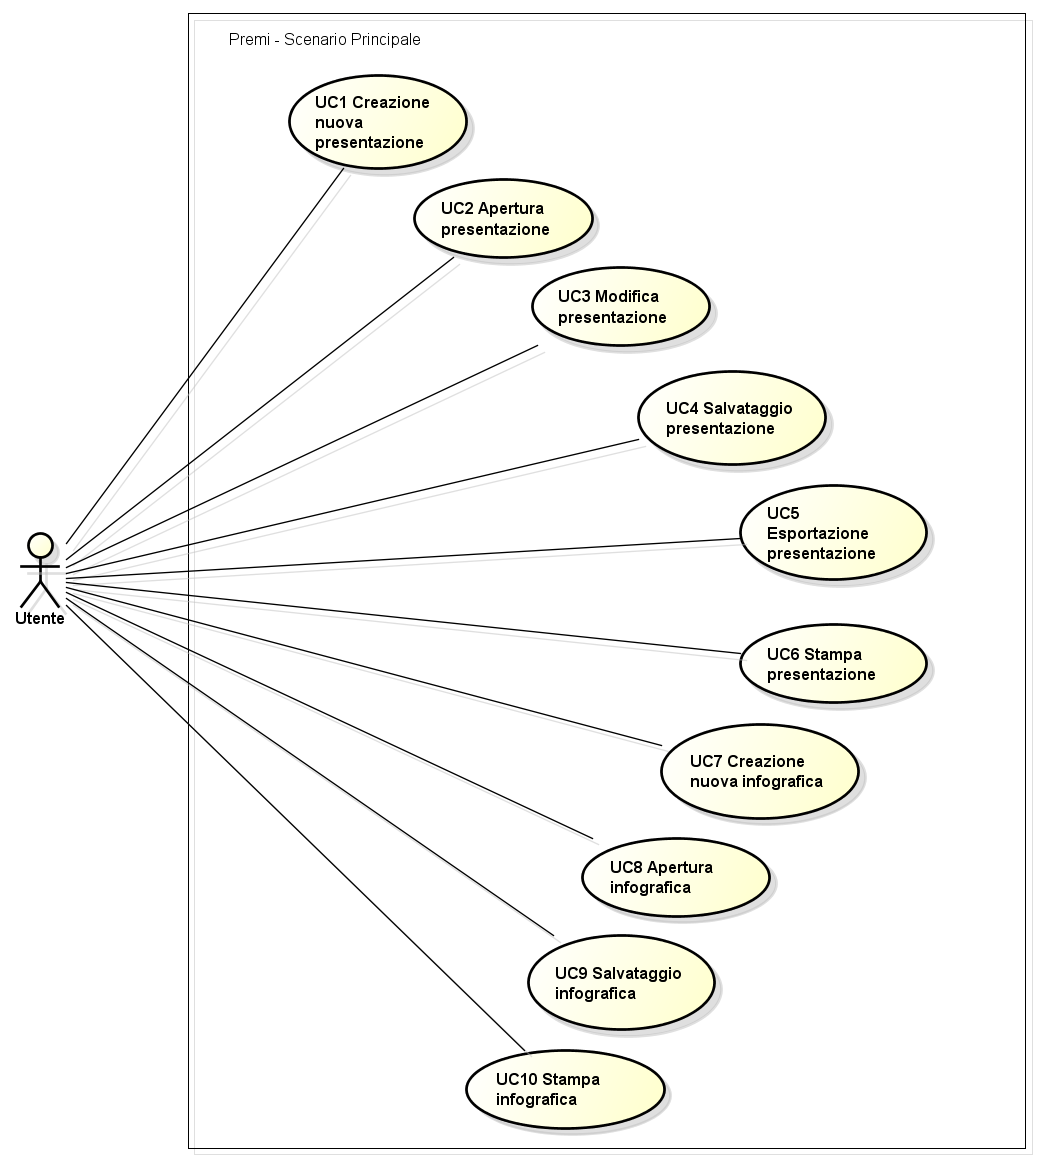
\includegraphics[scale=0.3] {img/UCP.png} 
	\caption{UCP - Scenario principale} 
\end{figure}

\begin{itemize}
	\item \textbf{Attori:} Utente non autenticato, Utente autenticato, Utente proprietario;
	
	\item \textbf{Scopo e descrizione:} Un visualizzatore può interagire con un progetto già esistente, senza però poterlo modificare. Il proprietario invece, dopo essersi autenticato, potrà effettuare diverse operazioni. Potrà creare nuovo progetto, modificarlo, salvarla oppure esportarlo per renderlo disponibile offline. Potrà inoltre generare il PDF rispettivo PDF per poi stamparlo o salvarlo.
	
	\item \textbf{Precondizione:} Il visualizzatore ha a disposizione una progetto con il quale interagire oppure il proprietario ha avviato il programma che ora è pronto all'uso;
	
	\item \textbf{Flusso principale degli eventi:}
	\begin{enumerate}
		\item L'utente si registra [UC1];
		\item L'utente si autentica [UC2];
		\item L'utente ricerca un progetto [UC3];
		\item L'utente visualizza un progetto [UC4];
		\item L'utente genera il file PDF del progetto [UC5];
		\item L'utente esporta un progetto [UC6];
		\item L'utente crea un nuovo progetto [UC7];
		\item L'utente proprietario apre un progetto esistente [UC8];
		\item L'utente proprietario modifica un progetto [UC9];
		\item L'utente proprietario crea un'\gls{infografica} [UC10];
		\item L'utente proprietario salva il progetto [UC11];
		\item L'utente proprietario elimina un progetto [UC12].
	\end{enumerate}
	
	\item \textbf{Postcondizione:} Il sistema ha ottenuto le informazioni sulle operazioni che il visualizzatore o il proprietario desidera eseguire.
\end{itemize}

\newpage
\subsection{Caso d'uso UC1: Registrazione}
\begin{figure}[h] 
	\centering 
	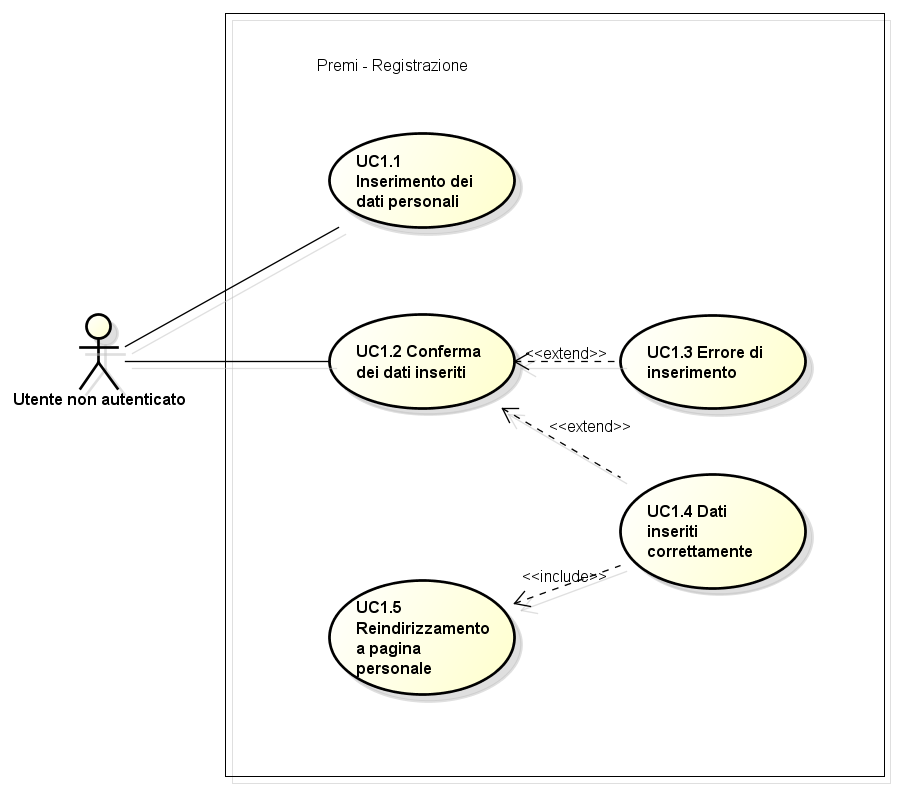
\includegraphics[scale=0.45] {img/UC1.png} 
	\caption{UC1 - Registrazione} 
\end{figure}

\begin{itemize}
	\item \textbf{Attori:} Utente non autenticato;
	\item \textbf{Scopo e descrizione:} L'utente non è iscritto e vuole avviare la procedura di iscrizione al sito;
	\item \textbf{Precondizione:} L'utente ha selezionato la voce "registrati" presente sul sito;
	\item \textbf{Flusso principale degli eventi:}
	\begin{enumerate}
		\item L'utente inserisce i propri dati personali [UC1.1];
		\item L'utente conferma l'inserimento dei propri dati [UC1.2];
		\item Si può verificare un errore di inserimento [UC1.3];
		\item I dati sono stati inseriti correttamente [UC1.4];
		\item Il sistema reindirizza l'utente alla sua pagina personale [UC1.5];
	\end{enumerate}
	\item \textbf{Postcondizione:} Il sistema ha registrato il nuovo utente e lo ha reindirizzato alla propria pagina personale.
\end{itemize}

\newpage

\subsection{Caso d'uso UC1.1: Inserimento dati personali}
\begin{figure}[h] 
	\centering 
	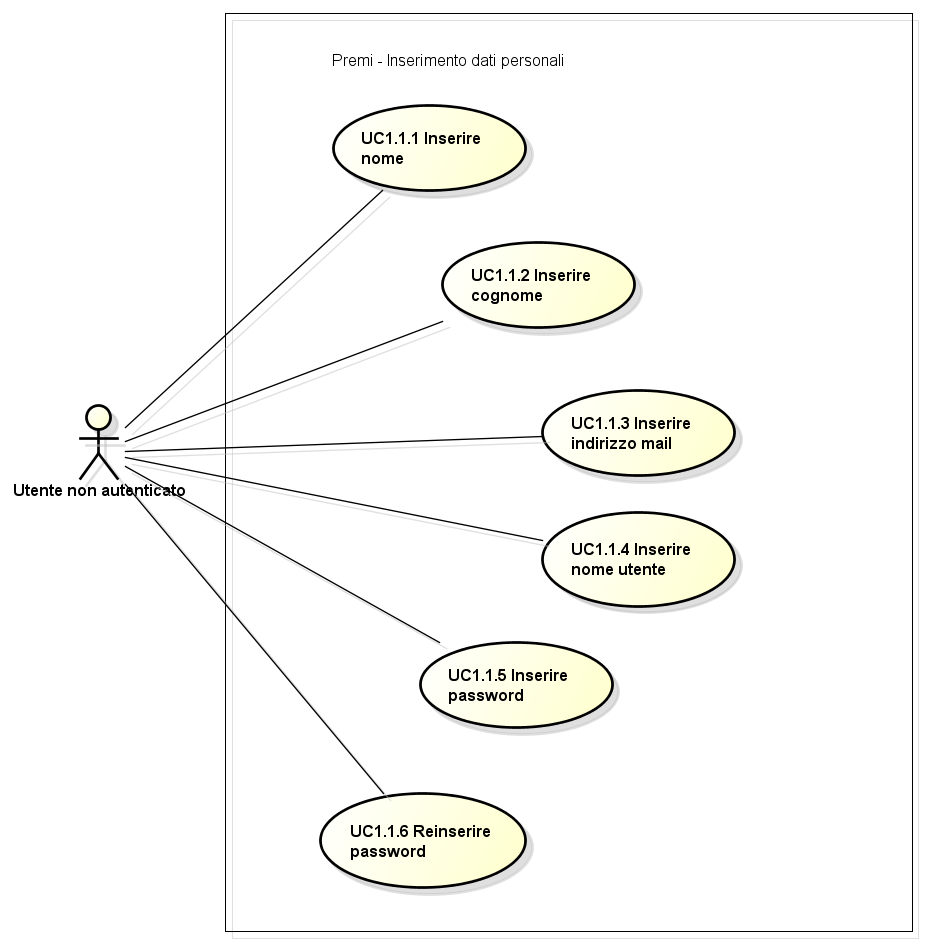
\includegraphics[scale=0.45] {img/UC1.1.png} 
	\caption{UC1.1 - Inserimento dati personali} 
\end{figure}
\begin{itemize}
	\item \textbf{Attori:} Utente non autenticato;
	\item \textbf{Scopo e descrizione:} L'utente inserisce tutti i dati richiesti per la registrazione;
	\item \textbf{Precondizione:} L'utente visualizza la schermata di inserimento dei dati richiesti per la registrazione;
	\item \textbf{Flusso principale degli eventi:}
	\begin{enumerate}
		\item L'utente inserisce il proprio nome [UC1.1.1];
		\item L'utente inserisce il proprio cognome [UC1.1.2];
		\item L'utente inserisce il proprio indirizzo mail [UC1.1.3];
		\item L'utente inserisce il proprio nome utente [UC1.1.4];
		\item L'utente inserisce una password [UC1.1.5];
		\item L'utente inserisce nuovamente la password [UC1.1.6].
	\end{enumerate}
	\item \textbf{Postcondizione:} Tutti i campi richiesti sono stati compilati correttamente.
\end{itemize}

\subsection{Caso d'uso UC1.1.1: Inserire nome}
\begin{itemize}
	\item \textbf{Attori:} Utente non autenticato;
	\item \textbf{Scopo e descrizione:} L'utente inserisce il proprio nome;
	\item \textbf{Precondizione:} La casella dove inserire il nome è vuota;
	\item \textbf{Postcondizione:} La casella è stata compilata con il nome inserito dall'utente.
\end{itemize}

\subsection{Caso d'uso UC1.1.2: Inserire cognome}
\begin{itemize}
	\item \textbf{Attori:} Utente non autenticato;
	\item \textbf{Scopo e descrizione:} L'utente inserisce il proprio cognome;
	\item \textbf{Precondizione:} La casella dove inserire il cognome è vuota;
	\item \textbf{Postcondizione:} La casella è stata compilata con il cognome inserito dall'utente.
\end{itemize}

\subsection{Caso d'uso UC1.1.3: Inserire indirizzo mail}
\begin{itemize}
	\item \textbf{Attori:} Utente non autenticato;
	\item \textbf{Scopo e descrizione:} L'utente inserisce il proprio indirizzo mail;
	\item \textbf{Precondizione:} La casella dove inserire l'indirizzo mail è vuota;
	\item \textbf{Postcondizione:} La casella è stata compilata con l'indirizzo mail inserito dall'utente.
\end{itemize}

\subsection{Caso d'uso UC1.1.4: Inserire nome utente}
\begin{itemize}
	\item \textbf{Attori:} Utente non autenticato;
	\item \textbf{Scopo e descrizione:} L'utente inserisce il proprio nome utente;
	\item \textbf{Precondizione:} La casella dove inserire il nome utente è vuota;
	\item \textbf{Postcondizione:} La casella è stata compilata con il nome utente inserito dall'utente.
\end{itemize}

\subsection{Caso d'uso UC1.1.5: Inserire password}
\begin{itemize}
	\item \textbf{Attori:} Utente non autenticato;
	\item \textbf{Scopo e descrizione:} L'utente inserisce la propria password;
	\item \textbf{Precondizione:} La casella dove inserire la password è vuota;
	\item \textbf{Postcondizione:} La casella è stata compilata con la password inserita dall'utente.
\end{itemize}

\subsection{Caso d'uso UC1.1.6: Reinserire password}
\begin{itemize}
	\item \textbf{Attori:} Utente non autenticato;
	\item \textbf{Scopo e descrizione:} L'utente inserisce nuovamente la password inserita in precedenza;
	\item \textbf{Precondizione:} La casella dove inserire la password è già stata compilata e la casella dove reinserire per la seconda volta la password è vuota;
	\item \textbf{Postcondizione:} La casella di reinserimento password è stata compilata con la password inserita dall'utente.
\end{itemize}

\subsection{Caso d'uso UC1.2: Conferma dei dati inseriti}
\begin{itemize}
	\item \textbf{Attori:} Utente non autenticato;
	\item \textbf{Scopo e descrizione:} L'utente deve confermare i dati inseriti in precedenza per procedere con l'iscrizione;
	\item \textbf{Precondizione:} L'utente ha inserito i dati richiesti per la registrazione;
	\item \textbf{Postcondizione:} Il sistema elabora i dati e registra il nuovo utente.
\end{itemize}

\subsection{Caso d'uso UC1.3: Errore di inserimento}
\begin{itemize}
	\item \textbf{Attori:} Sistema;
	\item \textbf{Scopo e descrizione:} Dopo che l'utente ha confermato i dati, il sistema segnala all'utente che c'è stato un errore di inserimento e mostra nuovamente la schermata di inserimento dei dati personali;
	\item \textbf{Precondizione:} L'utente ha confermato i dati inseriti;
	\item \textbf{Postcondizione:} Il sistema segnala all'utente che c'è stato un errore di inserimento e mostra di nuovo la schermata di inserimento dei dati personali.
\end{itemize}

\subsection{Caso d'uso UC1.4: Dati inseriti correttamente}
\begin{itemize}
	\item \textbf{Attori:} Sistema;
	\item \textbf{Scopo e descrizione:} Dopo che l'utente ha confermato i dati inseriti, il sistema li controlla e li accetta;
	\item \textbf{Precondizione:} L'utente ha confermato i dati inseriti;
	\item \textbf{Postcondizione:} Il sistema controlla e accetta i dati inseriti dall'utente.
\end{itemize}

\subsection{Caso d'uso UC1.5: Reindirizzamento a pagina personale}
\begin{itemize}
	\item \textbf{Attori:} Sistema;
	\item \textbf{Scopo e descrizione:} Dopo aver confermato i propri dati, il sistema reindirizza l'utente alla propria pagina personale dove può accedere alle varie funzionalità del sito;
	\item \textbf{Precondizione:} Il sistema ha registrato correttamente il nuovo utente;
	\item \textbf{Postcondizione:} Il sistema permette all'utente di visualizzare la propria pagina personale.
\end{itemize}	% registrazione
\newpage

\subsection{Caso d'uso UC2: Autenticazione}
\begin{figure}[h] 
	\centering 
	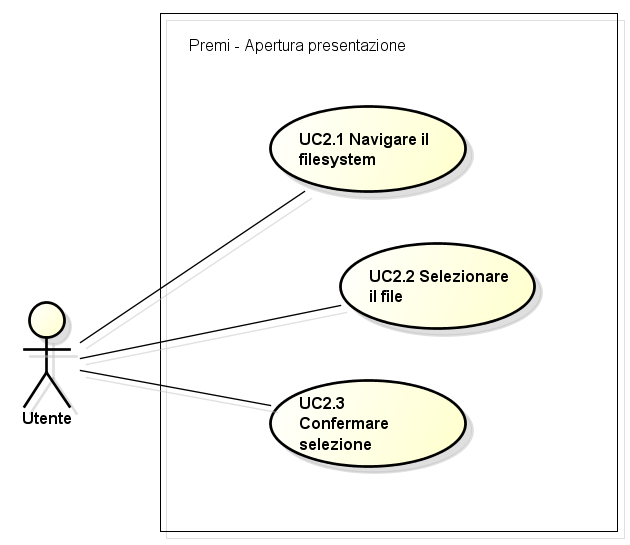
\includegraphics[scale=0.45] {img/UC2.png}
	\caption{UC2 - Autenticazione} 
\end{figure}

\begin{itemize}
	\item \textbf{Attori:} Utente non autenticato;
	\item \textbf{Scopo e descrizione:} L'utente è già iscritto e vuole avviare la procedura di autenticazione al sito per accedere ai propri file;
	\item \textbf{Precondizione:} L'utente ha selezionato la voce "accedi" presente sul sito;
	\item \textbf{Flusso principale degli eventi:}
	\begin{enumerate}
		\item L'utente inserisce le proprie credenziali [UC2.1];
		\item L'utente conferma l'inserimento dei dati selezionando la voce "login" [UC2.2];
		\item Si può verificare un errore di accesso [UC2.3];
		\item Il sistema controlla i dati inseriti e li accetta [UC2.4];
		\item L'utente viene reindirizzato alla propria pagina personale [UC2.5];
		\item L'utente può recuperare le sue credenziali se le dimentica [UC2.6].
	\end{enumerate}
	\item \textbf{Postcondizione:} Il sistema verifica le credenziali inserite e permette all'utente di accedere alla sua pagina personale.
\end{itemize}

\subsection{Caso d'uso UC2.1: Inserimento credenziali}
\begin{figure}[h] 
	\centering 
	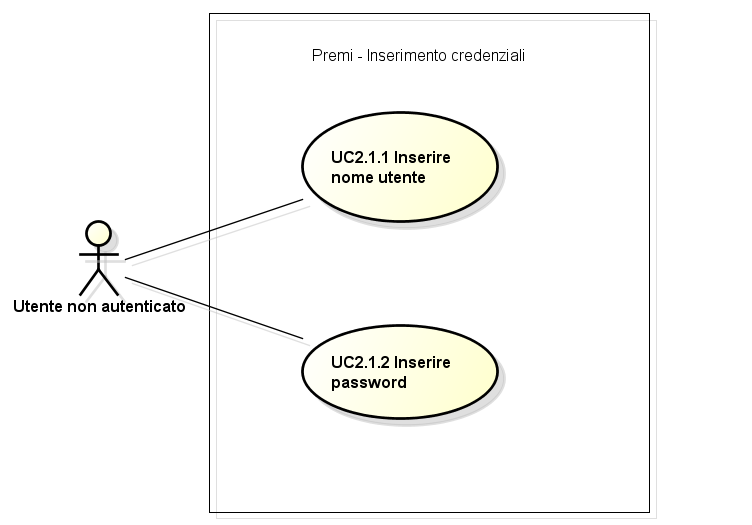
\includegraphics[scale=0.45] {img/UC2.1.png}
	\caption{UC2.1 - Inserimento credenziali} 
\end{figure}
\begin{itemize}
	\item \textbf{Attori:} Utente non autenticato;
	\item \textbf{Scopo e descrizione:} L'utente inserisce nome utente e password per poter accedere al sito;
	\item \textbf{Precondizione:} L'utente visualizza la schermata di inserimento dei dati richiesti per l'accesso;
	\item \textbf{Flusso principale degli eventi:}
	\begin{enumerate}
		\item L'utente inserisce il proprio nome utente [UC2.1.1];
		\item L'utente inserisce la propria password [UC2.1.2];
	\end{enumerate}
	\item \textbf{Postcondizione:} Tutti i campi richiesti sono stati compilati correttamente.
\end{itemize}

\subsection{Caso d'uso UC2.1.1: Inserire nome utente}
\begin{itemize}
	\item \textbf{Attori:} Utente non autenticato;
	\item \textbf{Scopo e descrizione:} L'utente inserisce il proprio nome utente;
	\item \textbf{Precondizione:} La casella dove inserire il nome utente è vuota;
	\item \textbf{Postcondizione:} La casella è stata compilata con il nome utente inserito dall'utente.
\end{itemize}

\subsection{Caso d'uso UC2.1.2: Inserire password}
\begin{itemize}
	\item \textbf{Attori:} Utente non autenticato;
	\item \textbf{Scopo e descrizione:} L'utente inserisce la propria password;
	\item \textbf{Precondizione:} La casella dove inserire la password è vuota;
	\item \textbf{Postcondizione:} La casella è stata compilata con la password inserita dall'utente.
\end{itemize}

\subsection{Caso d'uso UC2.2: Accesso}
\begin{itemize}
	\item \textbf{Attori:} Utente non autenticato;
	\item \textbf{Scopo e descrizione:} L'utente conferma le credenziali inserite scegliendo di effettuare l'accesso tramite il tasto di login;
	\item \textbf{Precondizione:} Nome utente e password sono stati inseriti;
	\item \textbf{Postcondizione:} Il sistema verifica i dati inseriti.
\end{itemize}

\subsection{Caso d'uso UC2.3: Errore di autenticazione}
\begin{itemize}
	\item \textbf{Attori:} Sistema;
	\item \textbf{Scopo e descrizione:} L'utente ha inserito delle credenziali errate e il sistema blocca l'accesso, riportando l'utente alla schermata di accesso;
	\item \textbf{Precondizione:} Nome utente e password sono stati inseriti in modo errato;
	\item \textbf{Postcondizione:} Il sistema riporta l'utente alla schermata di accesso.
\end{itemize}

\subsection{Caso d'uso UC2.4: Dati inseriti correttamente}
\begin{itemize}
	\item \textbf{Attori:} Sistema;
	\item \textbf{Scopo e descrizione:} Il sistema ha verificato che le credenziali inserite sono corrette;
	\item \textbf{Precondizione:} Nome utente e password sono stati inseriti;
	\item \textbf{Postcondizione:} Il sistema ha verificato che i dati inseriti sono corretti.
\end{itemize}

\subsection{Caso d'uso UC2.5: Reindirizzamento a pagina personale}
\begin{itemize}
	\item \textbf{Attori:} Sistema;
	\item \textbf{Scopo e descrizione:} Il sistema dopo aver consentito l'accesso all'utente mostra la sua pagina personale;
	\item \textbf{Precondizione:} Nome utente e password sono stati inseriti correttamente;
	\item \textbf{Postcondizione:} Il sistema mostra la pagina personale dell'utente.
\end{itemize}

\subsection{Caso d'uso UC2.6: Recupero dati}
\begin{figure}[h] 
	\centering 
	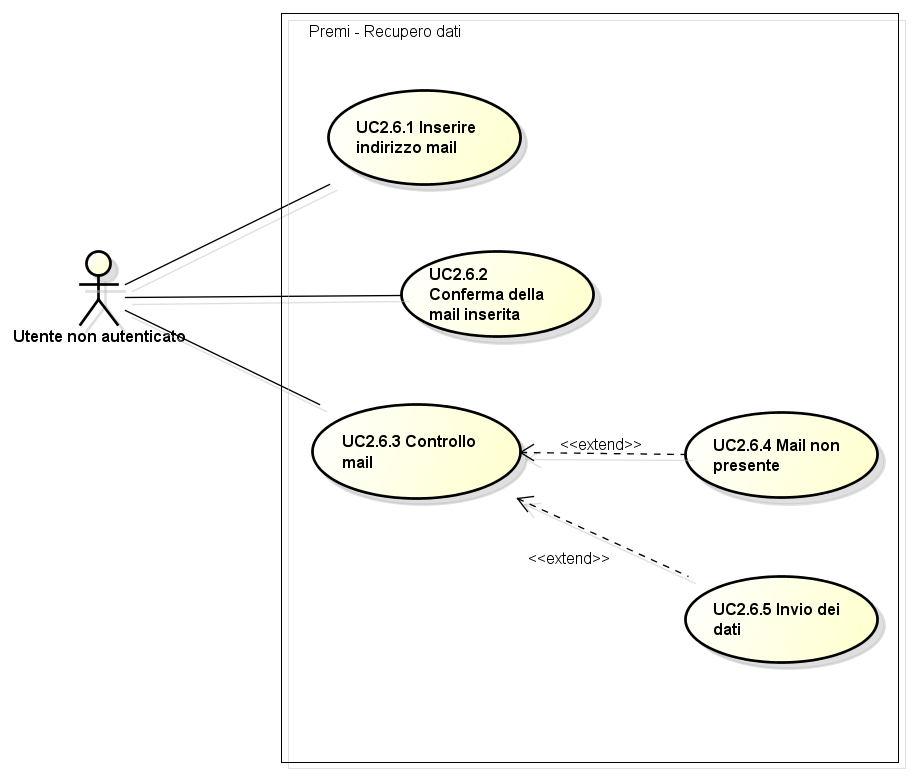
\includegraphics[scale=0.45] {img/UC2.6.png}
	\caption{UC2.6 - Recupero dati} 
\end{figure}
\begin{itemize}
	\item \textbf{Attori:} Utente non autenticato;
	\item \textbf{Scopo e descrizione:} L'utente non ricorda più le sue credenziali di accesso e sceglie quindi l'opzione per il recupero di tali dati. Il sistema gestirà la richiesta inviando all'indirizzo e-mail dell'utente tutti i suoi dati;
	\item \textbf{Precondizione:} L'utente ha selezionato l'opzione di recupero dei dati;
	\item \textbf{Flusso principale degli eventi:}
	\begin{enumerate}
		\item L'utente inserisce il proprio indirizzo mail [UC2.6.1];
		\item L'utente conferma l'inserimento dell'indirizzo mail [UC2.6.2];
		\item Il sistema controlla l'indirizzo e-mail inserita [UC2.6.3];
		\item Il sistema non trova l'indirizzo e-mail nel \gls{database} e segnala un errore [2.6.4];
		\item Il sistema trova una corrispondenza con l'indirizzo e-mail indicato e invia i dati [2.6.5].
	\end{enumerate}
	\item \textbf{Postcondizione:} Il sistema ha inviato una mail contenente i dati di accesso relativi all'utente che ne ha fatto richiesta.
\end{itemize}

\subsection{Caso d'uso UC2.6.1: Inserire indirizzo mail}
\begin{itemize}
	\item \textbf{Attori:} Utente non autenticato;
	\item \textbf{Scopo e descrizione:} L'utente inserisce il proprio indirizzo e-mail nella casella vuota;
	\item \textbf{Precondizione:} La casella dove inserire l'indirizzo e-mail è vuota;
	\item \textbf{Postcondizione:} La casella è stata compilata con l'indirizzo e-mail inserito dall'utente.
\end{itemize}

\subsection{Caso d'uso UC2.6.2: Conferma della mail inserita}
\begin{itemize}
	\item \textbf{Attori:} Utente non autenticato;
	\item \textbf{Scopo e descrizione:} L'utente conferma la mail inserita in precedenza e invia la richiesta;
	\item \textbf{Precondizione:} L'utente ha inserito un indirizzo e-mail;
	\item \textbf{Postcondizione:} L'utente ha confermato l'indirizzo e-mail inserito.
\end{itemize}

\subsection{Caso d'uso UC2.6.3: Controllo mail}
\begin{itemize}
	\item \textbf{Attori:} Sistema;
	\item \textbf{Scopo e descrizione:} Il sistema controlla che l'e-mail inserita dall'utente sia già presente nel \gls{database};
	\item \textbf{Precondizione:} L'utente ha confermato l'inserimento del proprio indirizzo e-mail;
	\item \textbf{Postcondizione:} Il sistema ha controllato che l'indirizzo e-mail inserito esista nel \gls{database}.
\end{itemize}

\subsection{Caso d'uso UC2.6.4: Indirizzo e-mail non presente}
\begin{itemize}
	\item \textbf{Attori:} Sistema;
	\item \textbf{Scopo e descrizione:} Il sistema non trova l'indirizzo e-mail nel \gls{database} e lo segnala all'utente;
	\item \textbf{Precondizione:} Il sistema ha controllato l'indirizzo e-mail inserito e non ha trovato corrispondenze nel \gls{database};
	\item \textbf{Postcondizione:} Il sistema avvisa l'utente che l'e-mail inserita non esiste nel \gls{database}.
\end{itemize}

\subsection{Caso d'uso UC2.6.5: Invio dei dati}
\begin{itemize}
	\item \textbf{Attori:} Sistema;
	\item \textbf{Scopo e descrizione:} Il sistema ha trovato l'indirizzo e-mail nel \gls{database} e invia le credenziali alla mail dell'utente;
	\item \textbf{Precondizione:} Il sistema ha controllato l'indirizzo e-mail inserito e ha trovato una corrispondenza nel \gls{database};
	\item \textbf{Postcondizione:} Il sistema invia le credenziali all'indirizzo e-mail indicata all'utente e avvisa l'utente dell'avvenuto invio.
\end{itemize}

	% autenticazione
\newpage

\subsection{Caso d'uso UC3: Ricerca di un progetto}
\begin{figure}[h] 
	\centering 
	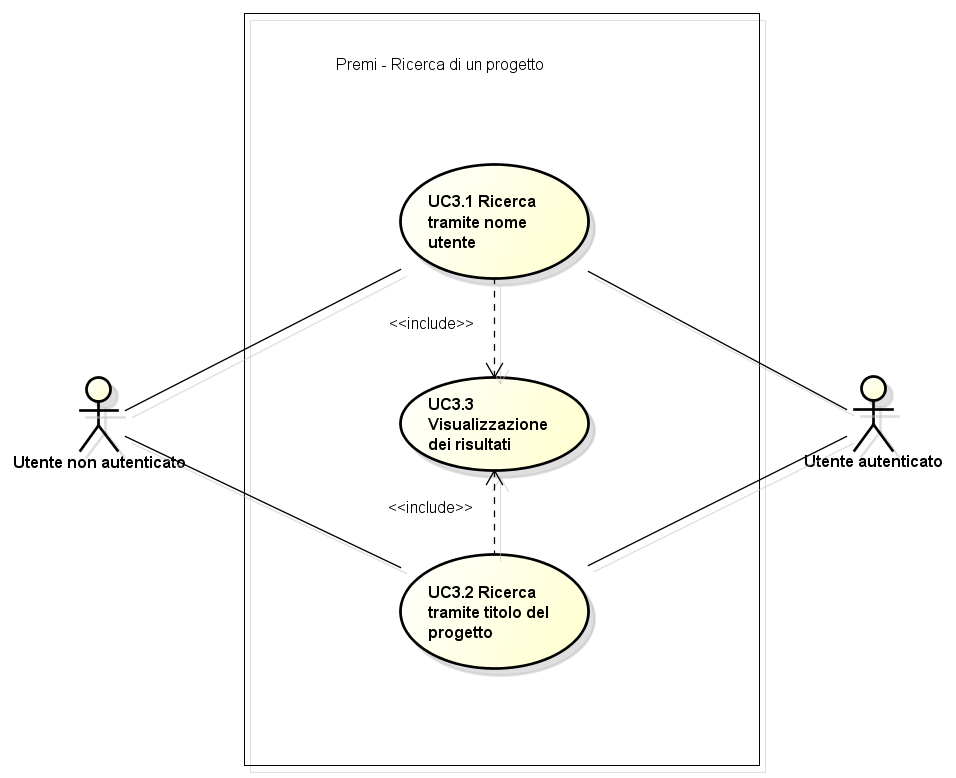
\includegraphics[scale=0.45] {img/UC3.png} 
	\caption{UC3 - Ricerca di un progetto} 
\end{figure}

\begin{itemize}
	\item \textbf{Attori:} Utente non autenticato, utente autenticato;
	\item \textbf{Scopo e descrizione:} L'utente può cercare un progetto utilizzando come chiave di ricerca il nome utente o il titolo del progetto;
	\item \textbf{Precondizione:} L'utente sta visualizzando la schermata di ricerca;
	\item \textbf{Flusso principale degli eventi:}
	\begin{enumerate}
		\item Ricerca tramite nome utente [UC3.1]
		\item Ricerca tramite titolo del progetto [UC3.2]
	\end{enumerate}
	\item \textbf{Postcondizione:} Il sistema mostra all'utente il risultato della ricerca visualizzando l'anteprima, il titolo e l'autore per ogni progetto.
\end{itemize}

\subsection{Caso d'uso UC3.1: Ricerca tramite nome utente}
\begin{itemize}
	\item \textbf{Attori:} Utente non autenticato, utente autenticato;
	\item \textbf{Scopo e descrizione:} L'utente inserisce nella casella di ricerca il nome utente di un creatore di un progetto;
	\item \textbf{Precondizione:} L'utente sta visualizzando la schermata di ricerca. Estende il caso d'uso UC3;
	\item \textbf{Postcondizione:} L'utente ha inserito un nome utente nella casella di ricerca ed ha avviato la ricerca.
\end{itemize}

\subsection{Caso d'uso UC3.2: Ricerca tramite titolo del progetto}
\begin{itemize}
	\item \textbf{Attori:} Utente non autenticato, utente autenticato;
	\item \textbf{Scopo e descrizione:} L'utente inserisce nella casella di ricerca il titolo di un progetto;
	\item \textbf{Precondizione:} L'utente sta visualizzando la schermata di ricerca. Estende il caso d'uso UC3;
	\item \textbf{Postcondizione:} L'utente ha inserito un titolo nella casella di ricerca ed ha avviato la ricerca.
\end{itemize}
	% ricerca
\newpage

\subsection{Caso d'uso UC4: Visualizzazione}
\begin{figure}[h] 
	\centering 
	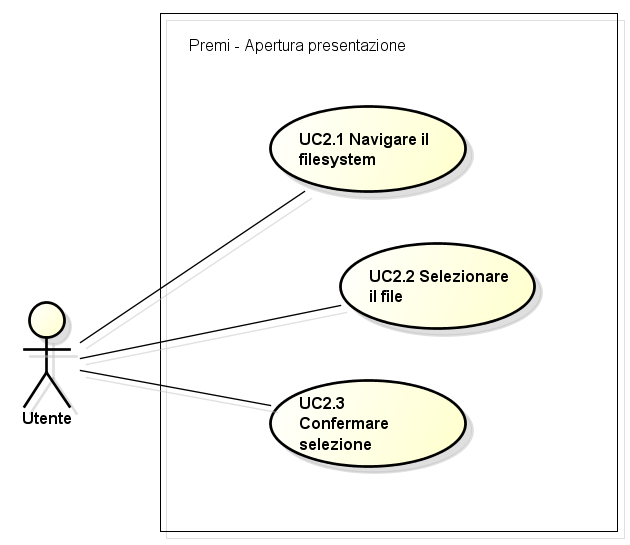
\includegraphics[scale=0.45] {img/UC4.png}
	\caption{UC4 - Visualizzazione} 
\end{figure}

\begin{itemize}
	\item \textbf{Attori:} Utente non autenticato, utente autenticato;
	\item \textbf{Scopo e descrizione:} Un utente, una volta aperto un progetto, può scegliere se visualizzare una presentazione o un'\gls{infografica};
	\item \textbf{Precondizione:} Il sistema mostra all'utente un progetto;
	\item \textbf{Flusso principale degli eventi:}
	\begin{enumerate}
		\item L'utente sceglie di visualizzare una presentazione [UC4.1];
		\item L'utente sceglie di visualizzare un'\gls{infografica} [UC4.2].
	\end{enumerate}
	\item \textbf{Postcondizione:} Il sistema mostra all'utente la schermata di visualizzazione di una presentazione o di un'\gls{infografica} a seconda di cosa è stato scelto.
\end{itemize}

\subsection{Caso d'uso UC4.1: Visualizzazione di una presentazione}
\begin{figure}[h] 
	\centering 
	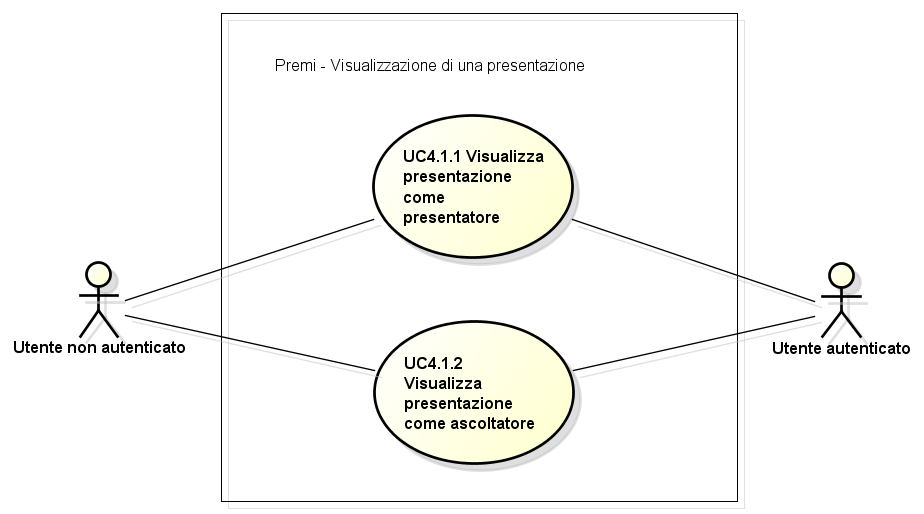
\includegraphics[scale=0.45] {img/UC4.1.png}
	\caption{UC4.1 - Visualizzazione di una presentazione} 
\end{figure}

\begin{itemize}
	\item \textbf{Attori:} Utente non autenticato, utente autenticato;
	\item \textbf{Scopo e descrizione:} La visualizzazione di una presentazione permette di scorrere le \gls{slide} nelle quattro direzioni a seconda di come sono state inserite. In generale, la presentazione segue un flusso principale (da sinistra a destra) nel quale sono presenti i capitoli principali, e un flusso secondario di dettaglio (dall'alto verso il basso) per ogni capitolo che si desidera, nel quale si può esplicitare l'argomento trattato.\\
	Durante il passaggio da un capitolo all'altro avverrà un effetto di "zoom-out, zoom-in" con il quale è possibile avere una panoramica della presentazione e soprattutto delle \gls{slide} del capitolo che si andrà ad affrontare.\\
	Una volta scelto di visualizzare una presentazione, l'utente può scegliere se visualizzarla come presentatore o come ascoltatore;
	\item \textbf{Precondizione:} L'utente ha scelto di visualizzare una presentazione;
	\item \textbf{Flusso principale degli eventi:}
	\begin{enumerate}
		\item L'utente sceglie di visualizzare la presentazione come presentatore [UC4.1.1];
		\item L'utente sceglie di visualizzare la presentazione come ascoltatore [UC4.1.2].
	\end{enumerate}
	\item \textbf{Postcondizione:} Il sistema mostra all'utente la schermata di visualizzazione di una presentazione con le impostazioni scelte.
\end{itemize}

\subsection{Caso d'uso UC4.1.1: Visualizzare una presentazione come presentatore}
\begin{itemize}
	\item \textbf{Attori:} Utente non autenticato, utente autenticato;
	\item \textbf{Scopo e descrizione:} L'utente ha scelto di visualizzare la presentazione come presentatore e il sistema mostra la presentazione con il supporto visivo dedicato al presentatore;
	\item \textbf{Precondizione:} L'utente ha scelto di visualizzare la presentazione come presentatore;
	\item \textbf{Postcondizione:} Il sistema avvia la presentazione con il supporto visivo dedicato al presentatore.
\end{itemize}

\subsection{Caso d'uso UC4.1.2: Visualizzare una presentazione come ascoltatore}
\begin{itemize}
	\item \textbf{Attori:} Utente non autenticato, utente autenticato;
	\item \textbf{Scopo e descrizione:} L'utente ha scelto di visualizzare la presentazione come ascoltatore e il sistema mostra la presentazione selezionata;
	\item \textbf{Precondizione:} L'utente ha scelto di visualizzare la presentazione come ascoltatore;
	\item \textbf{Postcondizione:} Il sistema avvia la presentazione.
\end{itemize}

\subsection{Caso d'uso UC4.2: Visualizzazione di un'infografica}
\begin{itemize}
	\item \textbf{Attori:} Utente non autenticato, utente autenticato;
	\item \textbf{Scopo e descrizione:} L'utente ha scelto di visualizzare un'\gls{infografica} e il sistema la mostra;
	\item \textbf{Precondizione:} L'utente ha scelto di visualizzare un'\gls{infografica};
	\item \textbf{Postcondizione:} Il sistema mostra all'utente la schermata di visualizzazione dell'\gls{infografica}.
\end{itemize}

	% visualizzazione
\newpage

\subsection{Caso d'uso UC5: Esportazione della presentazione}
	\begin{figure}[h] 
		\centering 
		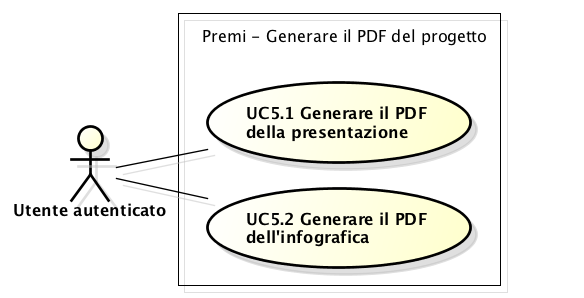
\includegraphics[scale=0.45] {img/UC5.png} 
		\caption{UC5 - Esportazione della presentazione} 
	\end{figure}
	
	\begin{itemize}
		\item \textbf{Attori:} Utente;
		\item \textbf{Scopo e descrizione:} L'utente ha creato una presentazione di slide e vuole esportarla in un formato diverso per salvarla nel proprio computer;
		\item \textbf{Precondizione:} Il sistema è in attesa che l'utente selezione la funzione esporta presentazione;
		\item \textbf{Flusso degli eventi:}
		\begin{enumerate}
			\item L'utente seleziona dal menù la funzione esporta [UC5.1];
			\item L'utente sceglie il formato in cui esportare la presentazione [UC5.2];
			\item L'utente sceglie dove esportare la presentazione [UC5.3];
			\item L'utente conferma l'esportazione [UC5.4];
		\end{enumerate}
		\item \textbf{Postcondizione:} Il sistema ha esportato la presentazione.
	\end{itemize}


\subsection{Caso d'uso UC5.1: Selezionare funzione esporta}
	\begin{itemize}
		\item \textbf{Attori:} Utente;
		\item \textbf{Scopo e descrizione:} L'utente seleziona dal menù la funzione esporta per esportare la presentazione;
		\item \textbf{Precondizione:} Il sistema è in attesa che l'utente selezioni la funzione dal menù;
		\item \textbf{Postcondizione:} Il sistema apre la finestra di dialogo per l'esportazione.
	\end{itemize}


\subsection{Caso d'uso UC5.2: Selezionare il formato di esportazione}
	\begin{itemize}
		\item \textbf{Attori:} Utente;
		\item \textbf{Scopo e descrizione:} L'utente deve scegliere il formato in cui esportare la presentazione;
		\item \textbf{Precondizione:} Il sistema è in attesa che l'utente selezioni il formato dall'apposita finestra di dialogo;
		\item \textbf{Postcondizione:} Il sistema registra la scelta e apre la finestra di dialogo per il salvataggio della presentazione esportata.
	\end{itemize}


\subsection{Caso d'uso UC5.3: Selezionare la destinazione di esportazione}
	\begin{itemize}
		\item \textbf{Attori:} Utente;
		\item \textbf{Scopo e descrizione:} L'utente deve scegliere la destinazione in cui salvare la presentazione esportata.
		\item \textbf{Precondizione:} Il sistema è in attesa che l'utente selezioni il percorso dall'apposita finestra di dialogo;
		\item \textbf{Postcondizione:} Il sistema registra la destinazione desiderata.
	\end{itemize}


\subsection{Caso d'uso UC5.4: Confermare l'esportazione}
	\begin{itemize}
		\item \textbf{Attori:} Utente;
		\item \textbf{Scopo e descrizione:} L'utente deve confermare l'esportazione della presentazione nel formato e nella destinazione desiderata;
		\item \textbf{Precondizione:} Il sistema è in attesa che l'utente confermi l'esportazione;
		\item \textbf{Postcondizione:} Il sistema ha esportato la presentazione.
	\end{itemize}
	
	
\subsection{Caso d'uso UC5.5: Selezionare il percorso}
	\begin{figure}[h] 
		\centering 
		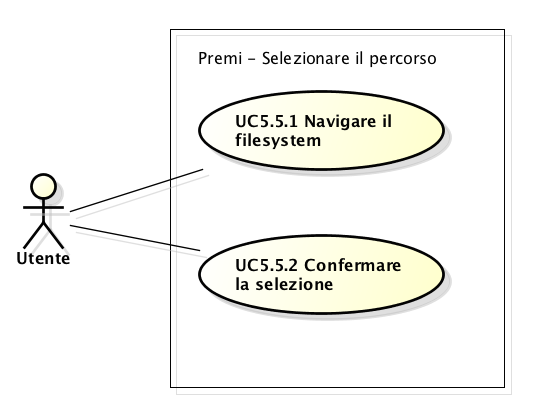
\includegraphics[scale=0.45] {img/UC5.5.png} 
		\caption{UC5.5 - Selezionare il percorso} 
	\end{figure}
	\begin{itemize}
		\item \textbf{Attori:} Utente;
		\item \textbf{Scopo e descrizione:} L'utente deve scegliere il percorso. Naviga il filesystem, lo seleziona ne e conferma la scelta;
		\item \textbf{Precondizione:} Il sistema è in attesa che l'utente navighi il filesystem e confermi il percorso scelto;
		\item \textbf{Flusso degli eventi:}
		\begin{enumerate}
			\item L'utente naviga il filesystem alla ricerca della posizione desiderata [UC5.5.1];
			\item L'utente conferma la posizione selezionata [UC5.5.2].
		\end{enumerate}
		\item \textbf{Postcondizione:} Il sistema registra il percorso desiderato.
	\end{itemize}
	
	\subsection{Caso d'uso UC5.5.1: Navigare il filesystem}
	\begin{itemize}
		\item \textbf{Attori:} Utente;
		\item \textbf{Scopo e descrizione:} L'utente può navigare il filesystem per selezionare la cartella dentro la quale vuole esportare la presentazione;
		\item \textbf{Precondizione:} Il sistema è in attesa che l'utente selezioni una cartella;
		\item \textbf{Postcondizione:} Il sistema ha aggiornato la il percorso con quello scelto dall'utente.
	\end{itemize}
	
	\subsection{Caso d'uso UC5.5.2: Confermare selezione}
	\begin{itemize}
		\item \textbf{Attori:} Utente;
		\item \textbf{Scopo e descrizione:} L'utente conferma che il percorso selezionato è quello corretto;
		\item \textbf{Precondizione:} Il sistema ha selezionato il percorso indicato dall'utente;
		\item \textbf{Postcondizione:} Il sistema ha registrato il percorso precedentemente scelto dall'utente.
	\end{itemize}	% generazione file PDF
\newpage

\subsection{Caso d'uso UC6: Esportazione del progetto}
	\begin{figure}[h]
		\centering
		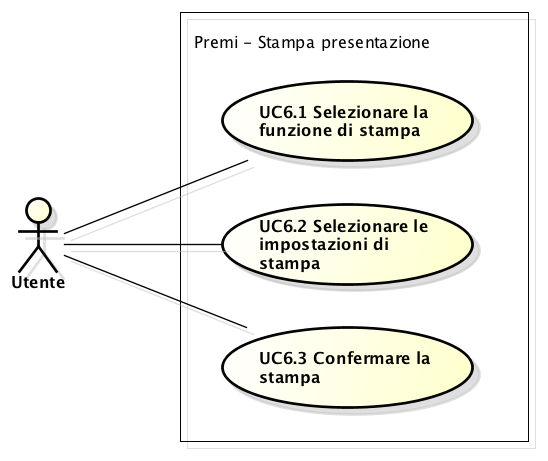
\includegraphics[scale=0.45] {img/UC6.png}
		\caption{UC6 - Esportazione del progetto}
	\end{figure}

	\begin{itemize}
		\item \textbf{Attori:} Utente autenticato, Proprietario;
		\item \textbf{Scopo e descrizione:} L'utente ha aperto un progetto e vuole esportarlo in locale per poterlo visualizzare offline;
		\item \textbf{Precondizione:} Il sistema è in attesa che l'utente selezioni la funzione esporta;
		\item \textbf{Flusso principale degli eventi:}
		\begin{enumerate}
			\item L'utente seleziona dal menù la funzione esporta [UC6.1];
			\item L'utente salva il pacchetto in locale [UC6.2].
		\end{enumerate}
		\item \textbf{Postcondizione:} L'utente ha esportato il progetto e l'ha salvato in locale.
	\end{itemize}


\subsection{Caso d'uso UC6.1: Selezionare la funzione esporta}
	\begin{itemize}
		\item \textbf{Attori:} Utente autenticato, Proprietario;
		\item \textbf{Scopo e descrizione:} L'utente seleziona dall'apposito menù la funzione di esportazione per esportare il progetto;
		\item \textbf{Precondizione:} L'utente ha un progetto aperto e il sistema è in attesa che l'utente selezioni la funzione esporta;
		\item \textbf{Postcondizione:} Il sistema inizia la procedura di esportazione.
	\end{itemize}


\subsection{Caso d'uso UC6.2: Salvataggio del pacchetto in locale}
	\begin{itemize}
		\item \textbf{Attori:} Utente autenticato, Proprietario;
		\item \textbf{Scopo e descrizione:} L'utente deve salvare il pacchetto del progetto in locale.
		\item \textbf{Precondizione:} Il sistema ha preparato il pacchetto, il quale è pronto per essere scaricato;
		\item \textbf{Postcondizione:} Il pacchetto è stato scaricato e salvato in locale dall'utente.
	\end{itemize}	% esportazione
\newpage

\subsection{Caso d'uso UC7: Creazione di un progetto}
\begin{figure}[h] 
	\centering 
	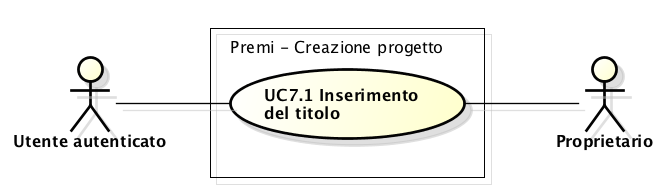
\includegraphics[scale=0.45] {img/UC7.png} 
	\caption{UC7 - Creazione di un progetto} 
\end{figure}

\begin{itemize}
	\item \textbf{Attori:} Utente autenticato, Proprietario;
	\item \textbf{Scopo e descrizione:} L'utente vuole creare un nuovo progetto. Ha la possibilità di decidere il titolo del progetto e il template con cui crearlo. Successivamente passerà alla fase di modifica.
	\item \textbf{Precondizione:} L'utente deve aver eseguito l'accesso al sistema;
	\item \textbf{Flusso principale degli eventi:}
	\begin{enumerate}
		\item L'utente sceglie il titolo [UC7.1];
		\item L'utente sceglie il template [UC7.2].
	\end{enumerate}
	\item \textbf{Postcondizione:} Il sistema registra le scelte dell'utente ed entra nella modalità di modifica.
\end{itemize}


\subsection{Caso d'uso UC7.1: Scegliere il titolo}
\begin{itemize}
	\item \textbf{Attori:} Utente autenticato, Proprietario;
	\item \textbf{Scopo e descrizione:} L'utente sceglie il titolo da dare al progetto;
	\item \textbf{Precondizione:} L'utente ha deciso di creare un nuovo progetto;
	\item \textbf{Postcondizione:} Il sistema registra il titolo inserito dall'utente.
\end{itemize}


\subsection{Caso d'uso UC7.2: Scegliere un template}
\begin{itemize}
	\item \textbf{Attori:} Utente autenticato, Proprietario;
	\item \textbf{Scopo e descrizione:} L'utente sceglie un template da utilizzare per il proprio progetto;
	\item \textbf{Precondizione:} L'utente ha inserito il titolo del progetto;
	\item \textbf{Postcondizione:} Il sistema crea una presentazione con il titolo e il template scelti e entra nella modalità di modifica.
\end{itemize}	% creazione progetto
\newpage

\subsection{Caso d'uso UC8: Apertura di un progetto}
\begin{itemize}
	\item \textbf{Attori:} Proprietario;
	\item \textbf{Scopo e descrizione:} L'utente vuole aprire un progetto esistente;
	\item \textbf{Precondizione:} L'utente ha selezionato un progetto già creato e salvato in precedenza;
	\item \textbf{Postcondizione:} Il sistema apre la schermata di modifica del progetto.
\end{itemize}
	% apertura
\newpage

\subsection{Caso d'uso UC9: Modifica della presentazione}
\begin{figure}[h] 
	\centering 
	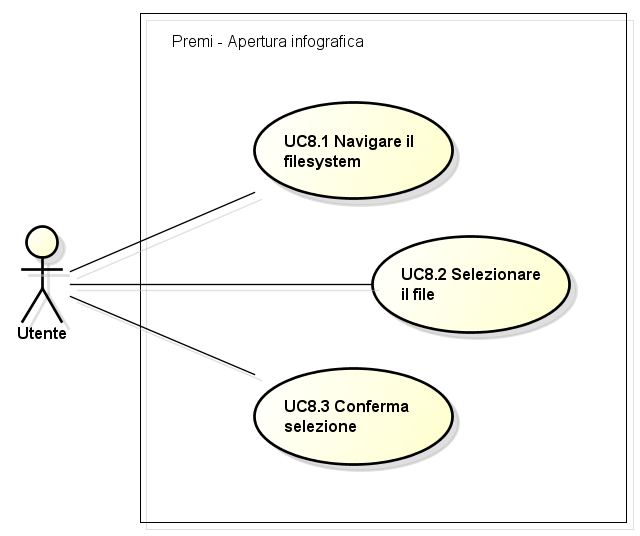
\includegraphics[scale=0.35] {img/UC9.png} 
	\caption{UC9 - Modifica della presentazione} 
\end{figure}

\begin{itemize}
	\item \textbf{Attori:} Proprietario;
	\item \textbf{Scopo e descrizione:} L'utente sta lavorando su una presentazione per inserire delle nuove slide o per modificare quelle già create. Può quindi inserire i seguenti elementi: slide, immagini, caselle di testo, dati real time, tabelle. Ha inoltre la possibilità di modificare gli elementi già inseriti, oppure di eliminarli. Può infine scegliere l'effetto di transizione tra una slide e l'altra;
	\item \textbf{Precondizione:} L'utente ha creato una presentazione nella fase di creazione di un progetto;
	\item \textbf{Flusso principale degli eventi:}
	\begin{enumerate}
		
		\item L'utente sceglie il template [UC9.1];
		
		\item L'utente inserisce una nuova slide [UC9.2];
		\item L'utente rimuove una slide [UC9.3];
		
		\item L'utente inserisce un'immagine [UC9.4];
		
		\item L'utente inserisce una casella di testo [UC9.5];
		
		\item L'utente inserisce dati real time [UC9.6];
		
		\item L'utente inserisce una tabella [UC9.7];
		
		\item L'utente inserisce un grafico [UC9.8];
		
		\item L'utente sceglie un effetto di transizione [UC9.9];
		
		\item L'utente cambia la dimensione di un elemento [UC9.10];
		
		\item L'utente cambia la posizione di un elemento [UC9.11];
		
		\item L'utente ruota un elemento [UC9.12];
		
		\item L'utente rimuove un elemento [UC9.13];
		
		\item L'utente carica un file per inserire l'immagine [UC9.14];
		\item L'utente sceglie la formattazione del testo [UC9.15];
		\item L'utente modifica una tabella [UC9.16];
		\item L'utente modifica un grafico [UC9.17];
		
		\item L'utente inserisce note / parole chiave [UC9.18].
	\end{enumerate}
	\item \textbf{Postcondizione:} Il sistema esegue le operazioni effettuate dall'utente.
\end{itemize}


\subsection{Caso d'uso UC9.1: Scegliere un template}
\begin{itemize}
	\item \textbf{Attori:} Proprietario;
	\item \textbf{Scopo e descrizione:} L'utente sceglie un template di stile da utilizzare per la propria presentazione;
	\item \textbf{Precondizione:} Il sistema è in attesa che l'utente selezioni il template da utilizzare;
	\item \textbf{Postcondizione:} Il sistema imposta il template selezionato per la presentazione.
\end{itemize}


\subsection{Caso d'uso UC9.2: Inserire una nuova slide}
\begin{itemize}
	\item \textbf{Attori:} Proprietario;
	\item \textbf{Scopo e descrizione:} L'utente crea una nuova slide nella presentazione per poter inserire del contenuto;
	\item \textbf{Precondizione:} Il sistema è in attesa che l'utente crei una nuova slide;
	\item \textbf{Postcondizione:} Il sistema ha creato la nuova slide.
\end{itemize}


\subsection{Caso d'uso UC9.3: Rimuovere una slide}
\begin{itemize}
	\item \textbf{Attori:} Proprietario;
	\item \textbf{Scopo e descrizione:} L'utente vuole rimuovere una slide della presentazione precedentemente creata;
	\item \textbf{Precondizione:} Il sistema è in attesa che l'utente selezioni una slide e il comando per rimuoverla;
	\item \textbf{Postcondizione:} Il sistema ha rimosso la slide selezionata.
\end{itemize}


\subsection{Caso d'uso UC9.4: Inserire un'immagine}
\begin{itemize}
\item \textbf{Attori:} Proprietario;
\item \textbf{Scopo e descrizione:} L'utente deve inserire un'immagine in una slide. Seleziona il comando e sceglie l'immagine da inserire nella slide corrente;
\item \textbf{Precondizione:} Il sistema è in attesa che l'utente selezioni il comando per inserire un'immagine;
\item \textbf{Postcondizione:} Il sistema ha inserito l'immagine selezionata dall'utente nella slide.
\end{itemize}


\subsection{Caso d'uso UC9.5: Inserire una casella di testo}
\begin{itemize}
\item \textbf{Attori:} Proprietario;
\item \textbf{Scopo e descrizione:} L'utente deve inserire una casella di testo nella slide. Seleziona il comando e inserisce la casella di testo nel punto della slide desiderato;
\item \textbf{Precondizione:} Il sistema è in attesa che l'utente selezioni il comando per inserire una casella di testo;
\item \textbf{Postcondizione:} Il sistema ha inserito la casella di testo nella slide.
\end{itemize}


\subsection{Caso d'uso UC9.6: Inserire dati real time}
\begin{itemize}
	\item \textbf{Attori:} Proprietario;
	\item \textbf{Scopo e descrizione:}	L'inserimento di un dato real time consiste nell'inserimento di una stringa speciale che si occuperà di richiamare dei contenuti personalizzabili definiti precedentemente dall'utente. Questi contenuti hanno il compito di catturare dati provenienti dall'esterno per poi riportarli nelle slide ed avere così dati aggiornati in tempo reale in quanto saranno composti di codice eseguito a run-time dal server. Nel caso la presentazione venga visualizzata offline, i contenuti faranno riferimento ai dati ottenuti nel momento dell'inserimento dell'oggetto.
	L'utente, quindi, deve inserire dei dati real time. Per inserirli deve caricare prima il codice che vuole richiamare attraverso l'oggetto inserito, poi inserire l'oggetto all'interno della presentazione indicando la funzione che deve svolgere.
	
	\item \textbf{Precondizione:} Il sistema è in attesa che l'utente inserisca i dati real time;
	\item \textbf{Flusso principale di eventi:}
	\begin{enumerate}
		\item L'utente inserisce il file contenente il codice da eseguire [UC9.6.1];
	\end{enumerate}
	\item \textbf{Postcondizione:} Il sistema ha inserito i dati real time.
\end{itemize}

	\subsection{Caso d'uso UC9.6.1: Inserire un file di codice}
	\begin{itemize}
		\item \textbf{Attori:} Proprietario;
		\item \textbf{Scopo e descrizione:} L'utente deve inserire un file di codice da usare per un oggetto di dati real time;
		\item \textbf{Precondizione:} Il sistema è in attesa che l'utente selezioni il comando per inserire un file;
		\item \textbf{Postcondizione:} Il sistema ha caricato il file nel server e lo ha inserito nella lista dei file di codice.
	\end{itemize}
	

\subsection{Caso d'uso UC9.7: Inserire una tabella}
\begin{itemize}
	\item \textbf{Attori:} Proprietario;
	\item \textbf{Scopo e descrizione:} L'utente deve inserire una tabella. Seleziona il numero di righe e di colonne e la inserisce nella posizione desiderata;
	\item \textbf{Precondizione:} Il sistema è in attesa che l'utente selezioni il comando per inserire una tabella nella slide;
	\item \textbf{Postcondizione:} Il sistema ha inserito la tabella nella slide e attiva la modalità di modifica della tabella.
\end{itemize}


\subsection{Caso d'uso UC9.8: Inserire un grafico}
\begin{figure}[h] 
	\centering 
	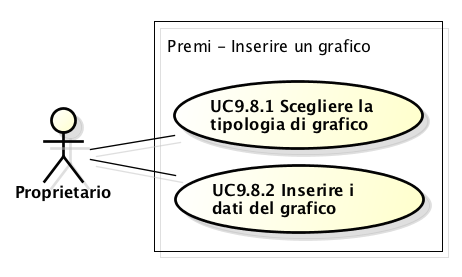
\includegraphics[scale=0.45] {img/UC9.8.png} 
	\caption{UC9.8 - Inserire grafico} 
\end{figure}

\begin{itemize}
	\item \textbf{Attori:} Proprietario;
	\item \textbf{Scopo e descrizione:} L'utente deve inserire un grafico. Seleziona il tipo di grafico e inserisce i dati;
	\item \textbf{Precondizione:} Il sistema è in attesa che l'utente selezioni il comando per inserire un grafico;
	\item \textbf{Flusso principale di eventi:}
	\begin{enumerate}
		\item L'utente sceglie la tipologia di grafico da inserire [UC9.8.1];
		\item L'utente inserisce i dati da inserire nel grafico [UC9.8.2];
	\end{enumerate}
	\item \textbf{Postcondizione:} Il sistema ha creato il grafico.
\end{itemize}

	\subsection{Caso d'uso UC9.8.1: Scegliere la tipologia del grafico}
	\begin{itemize}
		\item \textbf{Attori:} Proprietario;
		\item \textbf{Scopo e descrizione:} L'utente deve scegliere il tipo di grafico da inserire;
		\item \textbf{Precondizione:} Il sistema ha aperto la finestra di dialogo per la scelta del tipo di grafico;
		\item \textbf{Postcondizione:} Il sistema ha registrato la scelta dell'utente.
	\end{itemize}
	
	\subsection{Caso d'uso UC9.8.2: Inserire i dati del grafico}
	\begin{itemize}
		\item \textbf{Attori:} Proprietario;
		\item \textbf{Scopo e descrizione:} L'utente deve inserire i dati per il grafico da inserire;
		\item \textbf{Precondizione:} Il sistema è in attesa che l'utente inserisca ii dati;
		\item \textbf{Postcondizione:} Il sistema salva i dati inseriti.
	\end{itemize}


\subsection{Caso d'uso UC9.9: Scegliere un effetto di transizione}
\begin{itemize}
	\item \textbf{Attori:} Proprietario;
	\item \textbf{Scopo e descrizione:} L'utente deve scegliere l'effetto di transizione da dare alla slide;
	\item \textbf{Precondizione:} Il sistema è in attesa che l'utente selezioni l'effetto desiderato;
	\item \textbf{Postcondizione:} Il sistema ha inserito l'effetto di transizione.
\end{itemize}


\subsection{Caso d'uso UC9.10: Ridimensionamento di un elemento}
\begin{itemize}
	\item \textbf{Attori:} Proprietario;
	\item \textbf{Scopo e descrizione:} L'utente cambia la grandezza dell'elemento selezionato della slide;
	\item \textbf{Precondizione:} Il sistema mostra l'elemento selezionato che si intende ridimensionare;
	\item \textbf{Postcondizione:} Il sistema ha ridimensionato l'elemento della slide.
\end{itemize}


\subsection{Caso d'uso UC9.11: Spostamento di un elemento}
\begin{itemize}
	\item \textbf{Attori:} Proprietario;
	\item \textbf{Scopo e descrizione:} L'utente cambia la posizione dell'elemento selezionato della slide;
	\item \textbf{Precondizione:} Il sistema mostra l'elemento selezionato che si intende spostare;
	\item \textbf{Postcondizione:} Il sistema ha spostato l'elemento della slide.
\end{itemize}


\subsection{Caso d'uso UC9.12: Rotazione di un elemento}
\begin{itemize}
	\item \textbf{Attori:} Proprietario;
	\item \textbf{Scopo e descrizione:} L'utente ruota l'elemento selezionato della slide;
	\item \textbf{Precondizione:} Il sistema mostra l'elemento selezionato che si intende ruotare;
	\item \textbf{Postcondizione:} Il sistema ha ruotato l'elemento della slide.
\end{itemize}


\subsection{Caso d'uso UC9.13: Rimozione di un elemento}
\begin{itemize}
	\item \textbf{Attori:} Proprietario;
	\item \textbf{Scopo e descrizione:} L'utente elimina l'elemento selezionato dalla slide;
	\item \textbf{Precondizione:} Il sistema mostra l'elemento selezionato che si intende cancellare;
	\item \textbf{Postcondizione:} Il sistema ha cancellato l'elemento dalla slide.
\end{itemize}


\subsection{Caso d'uso UC9.14: Caricamento di un file}
\begin{itemize}
	\item \textbf{Attori:} Proprietario;
	\item \textbf{Scopo e descrizione:} L'utente deve caricare un file da utilizzare nella presentazione;
	\item \textbf{Precondizione:} Il sistema è in attesa che l'utente selezioni il file;
	\item \textbf{Postcondizione:} Il sistema ha caricato il file selezionato dall'utente e lo ha inserito nella slide.
\end{itemize}


\subsection{Caso d'uso UC9.15: Scegliere la formattazione del testo}
\begin{figure}[h] 
	\centering 
	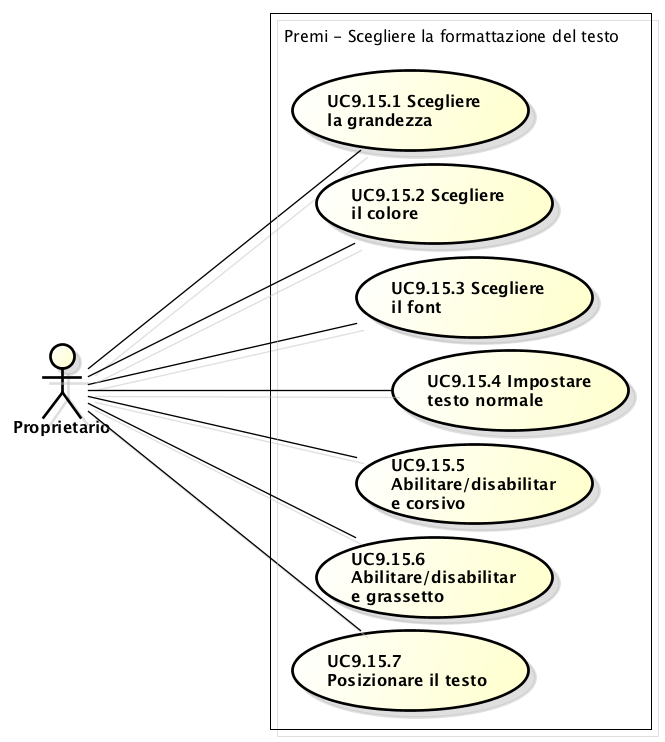
\includegraphics[scale=0.45] {img/UC9.15.png} 
	\caption{UC9.15 - Scegliere la formattazione del testo}
\end{figure}

\begin{itemize}
	\item \textbf{Attori:} Proprietario;
	\item \textbf{Scopo e descrizione:} L'utente può modificare l'aspetto del testo contenuto in una casella di testo. L'utente seleziona il testo e poi sceglie che modifiche effettuare;
	\item \textbf{Precondizione:} Il sistema è in attesa che l'utente selezioni la modifica da apportare al testo e il testo da modificare è selezionato;
	\item \textbf{Flusso principale degli eventi:}
	\begin{enumerate}
		\item L'utente può cambiare la grandezza del testo [UC9.15.1];
		\item L'utente può cambiare il colore del testo [UC9.15.2];
		\item L'utente può cambiare il font del testo [UC9.15.3];
		\item L'utente può abilitare o disabilitare il testo in corsivo [UC9.15.4];
		\item L'utente può abilitare o disabilitare il testo in grassetto [UC9.15.5];
		\item L'utente può spostare il testo in una nuova posizione [UC9.15.6].
	\end{enumerate}
	\item \textbf{Postcondizione:} Il sistema ha apportato le modifiche scelte al testo.
\end{itemize}

\subsection{Caso d'uso UC9.15.1: Scegliere la grandezza}
\begin{itemize}
	\item \textbf{Attori:} Proprietario;
	\item \textbf{Scopo e descrizione:} L'utente può cambiare la grandezza del testo;
	\item \textbf{Precondizione:} Il testo da modificare è selezionato;
	\item \textbf{Postcondizione:} Il testo è stato ingrandito o rimpicciolito secondo la scelta dell'utente.
\end{itemize}

\subsection{Caso d'uso UC9.15.2: Scegliere il colore}
\begin{itemize}
	\item \textbf{Attori:} Proprietario;
	\item \textbf{Scopo e descrizione:} L'utente può cambiare il colore del testo;
	\item \textbf{Precondizione:} Il testo da modificare è selezionato;
	\item \textbf{Postcondizione:} Il testo è stato colorato secondo la scelta dell'utente.
\end{itemize}

\subsection{Caso d'uso UC9.15.3: Scegliere il font}
\begin{itemize}
	\item \textbf{Attori:} Proprietario;
	\item \textbf{Scopo e descrizione:} L'utente può cambiare il font del testo;
	\item \textbf{Precondizione:} Il testo da modificare è selezionato;
	\item \textbf{Postcondizione:} Il testo ha cambiato font secondo la scelta dell'utente.
\end{itemize}

\subsection{Caso d'uso UC9.15.4: Abilitare/disabilitare corsivo}
\begin{itemize}
	\item \textbf{Attori:} Proprietario;
	\item \textbf{Scopo e descrizione:} L'utente può abilitare o disabilitare la scrittura in corsivo;
	\item \textbf{Precondizione:} Il testo da modificare è selezionato oppure è stata selezionata la casella di testo nella quale poter scrivere;
	\item \textbf{Postcondizione:} Il testo è stato modificato secondo la scelta dell'utente.
\end{itemize}

\subsection{Caso d'uso UC9.15.5: Abilitare/Disabilitare grassetto}
\begin{itemize}
	\item \textbf{Attori:} Proprietario;
	\item \textbf{Scopo e descrizione:} L'utente può abilitare o disabilitare la scrittura in grassetto;
	\item \textbf{Precondizione:} Il testo da modificare è selezionato oppure è stata selezionata la casella di testo nella quale poter scrivere;
	\item \textbf{Postcondizione:} Il testo è stato modificato secondo la scelta dell'utente.
\end{itemize}

\subsection{Caso d'uso UC9.15.6: Posizionare il testo}
\begin{itemize}
	\item \textbf{Attori:} Proprietario;
	\item \textbf{Scopo e descrizione:} L'utente può spostare una casella di testo in una nuova posizione;
	\item \textbf{Precondizione:} La casella di testo da spostare è stata selezionata;
	\item \textbf{Postcondizione:} La casella di testo è stata spostata secondo la scelta dell'utente.
\end{itemize}

\subsection{Caso d'uso UC9.16: Modificare una tabella}
\begin{figure}[h] 
	\centering 
	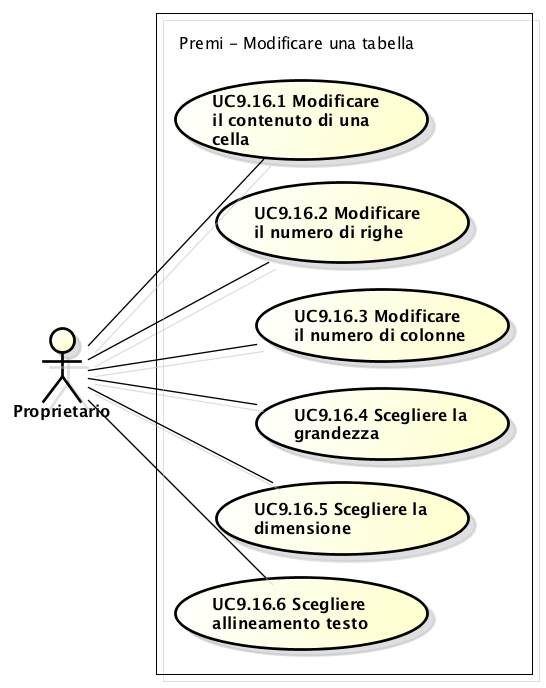
\includegraphics[scale=0.45] {img/UC9.16.png} 
	\caption{UC9.16 - Modificare una tabella} 
\end{figure}

\begin{itemize}
	\item \textbf{Attori:} Proprietario;
	\item \textbf{Scopo e descrizione:} L'utente può modificare l'aspetto della tabella e del suo contenuto. L'utente seleziona la tabella o il testo e poi sceglie che modifiche effettuare;
	\item \textbf{Precondizione:} Il sistema è in attesa che l'utente selezioni la modifica da apportare alla tabella e la tabella o il testo da modificare sono selezionati;
	\item \textbf{Flusso principale degli eventi:}
	\begin{enumerate}
		\item L'utente può modificare il contenuto di una cella [UC9.16.1];
		\item L'utente può modificare il numero di righe e di colonne [UC9.16.2];
		\item L'utente può cambiare la grandezza della tabella [UC9.16.3];
		\item L'utente può cambiare il colore di sfondo della tabella [UC9.16.4];
		\item L'utente può cambiare l'allineamento del testo [UC9.16.5];
		\item L'utente può cambiare la formattazione del testo [UC9.15];
	\end{enumerate}
	\item \textbf{Postcondizione:} Il sistema ha apportato le modifiche scelte alla tabella.
\end{itemize}

	\subsection{Caso d'uso UC9.16.1: Modificare il contenuto di una cella della tabella}
	\begin{itemize}
		\item \textbf{Attori:} Proprietario;
		\item \textbf{Scopo e descrizione:} L'utente può modificare il contenuto di una cella della tabella, cioè aggiungere e modificare elementi di testo;
		\item \textbf{Precondizione:} La cella da modificare è stata selezionata;
		\item \textbf{Postcondizione:} Il contenuto della cella è stato modificato.
	\end{itemize}
	
	\subsection{Caso d'uso UC9.16.2: Modificare il numero di righe e colonne della tabella}
	\begin{itemize}
		\item \textbf{Attori:} Proprietario;
		\item \textbf{Scopo e descrizione:} L'utente può modificare la grandezza della tabella;
		\item \textbf{Precondizione:} La tabella da modificare è stata selezionata;
		\item \textbf{Postcondizione:} La tabella è stata modificata nelle sue dimensioni secondo la scelta dell'utente.
	\end{itemize}
	
	\subsection{Caso d'uso UC9.16.3: Scegliere grandezza della tabella}
	\begin{itemize}
		\item \textbf{Attori:} Proprietario;
		\item \textbf{Scopo e descrizione:} L'utente può modificare la grandezza della tabella;
		\item \textbf{Precondizione:} La tabella da modificare è stata selezionata;
		\item \textbf{Postcondizione:} La tabella è stata modificata nelle sue dimensioni secondo la scelta dell'utente.
	\end{itemize}
	
	\subsection{Caso d'uso UC9.16.4: Scegliere colore di sfondo della tabella}
	\begin{itemize}
		\item \textbf{Attori:} Proprietario;
		\item \textbf{Scopo e descrizione:} L'utente può modificare il colore di sfondo della tabella;
		\item \textbf{Precondizione:} La tabella o le celle da modificare sono state selezionate;
		\item \textbf{Postcondizione:} Lo sfondo della tabella o delle celle è stato modificato secondo la scelta dell'utente.
	\end{itemize}
	
	\subsection{Caso d'uso UC9.16.5: Scegliere allineamento del testo}
	\begin{itemize}
		\item \textbf{Attori:} Proprietario;
		\item \textbf{Scopo e descrizione:} L'utente può modificare l'allineamento del testo della tabella;
		\item \textbf{Precondizione:} La tabella o le celle da modificare sono state selezionate;
		\item \textbf{Postcondizione:} L'allineamento del testo della tabella o delle celle è stato modificato secondo la scelta dell'utente.
	\end{itemize}
	
	
	\subsection{Caso d'uso UC9.17: Personalizzare un grafico}
	\begin{figure}[h] 
		\centering 
		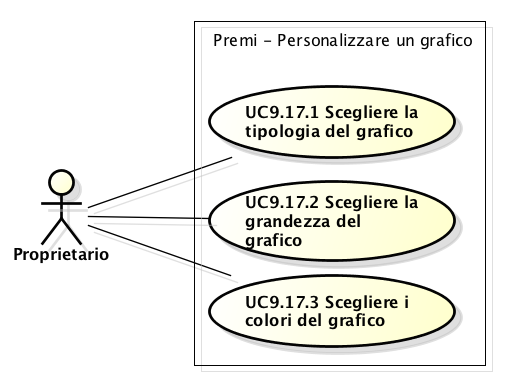
\includegraphics[scale=0.45] {img/UC9.17.png} 
		\caption{UC9.17 - Personalizzare un grafico} 
	\end{figure}
	
	\begin{itemize}
		\item \textbf{Attori:} Proprietario;
		\item \textbf{Scopo e descrizione:} L'utente può modificare la tipologia e l'aspetto del grafico o del suo contenuto. L'utente seleziona il grafico e poi sceglie che modifiche effettuare;
		\item \textbf{Precondizione:} Il sistema è in attesa che l'utente selezioni la modifica da apportare al grafico e il grafico da modificare è selezionato;
		\item \textbf{Flusso principale degli eventi:}
		\begin{enumerate}
			\item L'utente può cambiare la tipologia del grafico [UC9.17.1];
			\item L'utente può cambiare la dimensione del grafico [UC9.17.2]
			\item L'utente può cambiare i colori del grafico [UC9.17.3];
		\end{enumerate}
		\item \textbf{Postcondizione:} Il sistema ha apportato le modifiche scelte al grafico.
	\end{itemize}

		\subsection{Caso d'uso UC9.17.1: Scegliere la tipologia del grafico}
		\begin{itemize}
			\item \textbf{Attori:} Proprietario;
			\item \textbf{Scopo e descrizione:} L'utente deve modificare la tipologia del grafico. Seleziona il grafico e il comando per cambiare il tipo;
			\item \textbf{Precondizione:} Il grafico da modificare è stata selezionato e il sistema è in attesa che l'utente selezioni il comando;
			\item \textbf{Postcondizione:} La tipologia del grafico è stata modificata secondo la scelta dell'utente.
		\end{itemize}
		
		\subsection{Caso d'uso UC9.17.2: Scegliere la grandezza del grafico}
		\begin{itemize}
			\item \textbf{Attori:} Proprietario;
			\item \textbf{Scopo e descrizione:} L'utente deve modificare la grandezza del grafico;
			\item \textbf{Precondizione:} Il grafico da modificare è stata selezionato;
			\item \textbf{Postcondizione:} Il grafico è stata modificato nelle sue dimensioni secondo la scelta dell'utente.
		\end{itemize}
		
		\subsection{Caso d'uso UC9.17.3: Scegliere i colori del grafico}
		\begin{itemize}
			\item \textbf{Attori:} Proprietario;
			\item \textbf{Scopo e descrizione:} L'utente deve modificare il set di colori del grafico;
			\item \textbf{Precondizione:} Il grafico da modificare è stata selezionato e il sistema è in attesa che l'utente selezioni il comando;
			\item \textbf{Postcondizione:} I colori del grafico sono stati modificati secondo la scelta dell'utente.
		\end{itemize}


\subsection{Caso d'uso UC9.18: Inserire note / parole chiave}
\begin{itemize}
	\item \textbf{Attori:} Proprietario;
	\item \textbf{Scopo e descrizione:} L'utente deve inserire delle note o delle parole chiave nella slide da usare durante la visualizzazione della presentazione in modalità presentatore. Seleziona il comando e inserisce ciò che desidera includere;
	\item \textbf{Precondizione:} Il sistema è in attesa che venga selezionato il comando per inserire una nota / parola chiave;
	\item \textbf{Postcondizione:} Il sistema inserisce le note / parole chiave che l'utente ha aggiunto.
\end{itemize}	% modifica
\newpage

\subsection{Caso d'uso UC10: Stampa infografica}
\begin{figure}[h] 
	\centering 
	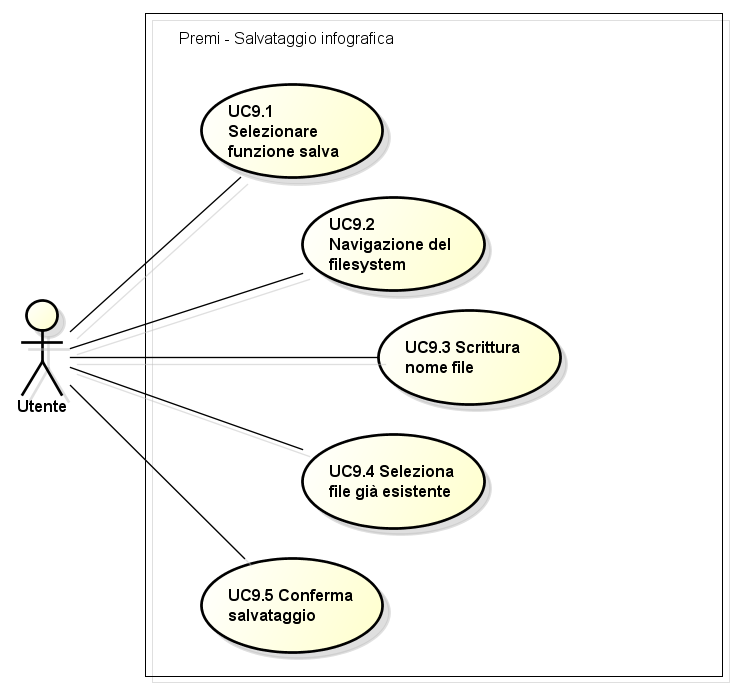
\includegraphics[scale=0.45] {img/UC10.png} 
	\caption{UC10 - Stampa infografica} 
\end{figure}

\begin{itemize}
	\item \textbf{Attori:} Utente;
	\item \textbf{Scopo e descrizione:} L'utente ha creato un'infografica e vuole stamparla;
	\item \textbf{Precondizione:} Il sistema è in attesa che l'utente selezioni la funzione stampa;
	\item \textbf{Flusso degli eventi:}
	\begin{enumerate}
		\item L'utente seleziona la funzione stampa [UC10.1];
		\item L'utente seleziona le impostazioni di stampa [UC10.2];
		\item L'utente conferma la stampa [UC10.3].
	\end{enumerate}
	\item \textbf{Postcondizione:} Il sistema ha mandato in stampa l'infografica.
\end{itemize}

\subsection{Caso d'uso UC10.1: Selezionare la funzione di stampa}
\begin{itemize}
	\item \textbf{Attori:} Utente;
	\item \textbf{Scopo e descrizione:} L'utente seleziona dall'apposito menù la funzione di stampa per stampare l'infografica;
	\item \textbf{Precondizione:} Il sistema è in attesa che l'utente selezioni la funzione stampa;
	\item \textbf{Postcondizione:} Il sistema apre la finestra di dialogo per la stampa.
\end{itemize}

\subsection{Caso d'uso UC10.2: Selezionare le impostazioni di stampa}
\begin{figure}[h] 
	\centering 
	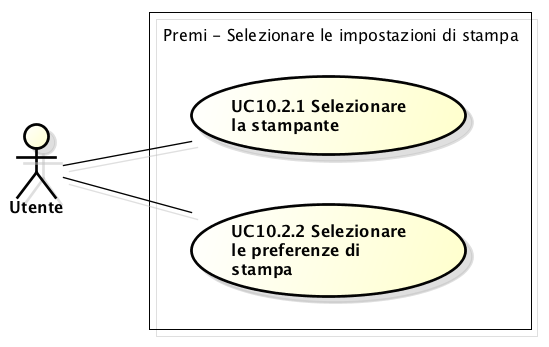
\includegraphics[scale=0.45] {img/UC10.2.png} 
	\caption{UC10.2 - Selezione impostazioni di stampa} 
\end{figure}

\begin{itemize}
	\item \textbf{Attori:} Utente;
	\item \textbf{Scopo e descrizione:} L'utente deve selezionare le impostazioni per la stampa dell'infografica;
	\item \textbf{Precondizione:} Il sistema permette all'utente di selezionare le impostazioni desiderate;
	\item \textbf{Flusso di eventi:}
	\begin{enumerate}
		\item L'utente seleziona quale stampante usare [UC10.2.1]
		\item L'utente seleziona le preferenze di stampa fornite dalla stampante[UC10.2.2]
	\end{enumerate}
	\item \textbf{Postcondizione:} Il sistema registra tutte le impostazioni selezionate dall'utente.
\end{itemize}
	
	\subsection{Caso d'uso UC10.2.1: Selezionare la stampante}
	\begin{itemize}
		\item \textbf{Attori:} Utente;
		\item \textbf{Scopo e descrizione:} L'utente seleziona quale stampante installata nel sistema usare;
		\item \textbf{Precondizione:} Il sistema è in attesa che l'utente selezioni la stampante da usare;
		\item \textbf{Postcondizione:} Il sistema registra la scelta fatta dall'utente.
	\end{itemize}
	
	\subsection{Caso d'uso UC10.2.2: Selezionare le preferenze di stampa}
	\begin{itemize}
		\item \textbf{Attori:} Utente;
		\item \textbf{Scopo e descrizione:} L'utente seleziona le preferenze di stampa fornite dai driver della stampante stessa;
		\item \textbf{Precondizione:} Il sistema è in attesa che l'utente selezioni le preferenze da usare;
		\item \textbf{Postcondizione:} Il sistema registra la scelte fatte dall'utente.
	\end{itemize}

\subsection{Caso d'uso UC10.3: Conferma di stampa}
\begin{itemize}
	\item \textbf{Attori:} Utente;
	\item \textbf{Scopo e descrizione:} L'utente conferma la stampa dell'infografica;
	\item \textbf{Precondizione:} Il sistema ha ricevuto la richiesta di stampa dell'infografica;
	\item \textbf{Postcondizione:} Il sistema ha mandato in stampa l'infografica.
\end{itemize}

\newpage	% creazione \gls{infografica}
\newpage

\subsection{Caso d'uso UC11: Salvataggio di un progetto}
\begin{figure}[h] 
	\centering 
	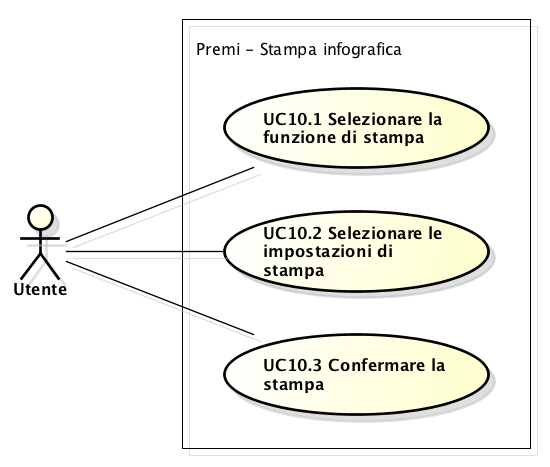
\includegraphics[scale=0.45] {img/UC11.png} 
	\caption{UC11 - Salvataggio di un progetto} 
\end{figure}

\begin{itemize}
	\item \textbf{Attori:} Proprietario;
	\item \textbf{Scopo e descrizione:} L'utente ha creato un progetto e vuole salvare il suo stato per poterlo aprire successivamente;
	\item \textbf{Precondizione:} L'utente ha creato un progetto nella fase di creazione;
	\item \textbf{Flusso principale degli eventi:}
	\begin{enumerate}
		\item L'utente seleziona la funzione salva [UC11.1];
		\item L'utente inserisce il nome del progetto [UC11.2];
	\end{enumerate}
	\item \textbf{Postcondizione:} Il sistema ha salvato il progetto nel server con il nome indicato dall'utente.
\end{itemize}


\subsection{Caso d'uso UC11.1: Selezionare la funzione salva}
\begin{itemize}
	\item \textbf{Attori:} Proprietario;
	\item \textbf{Scopo e descrizione:} L'utente seleziona dall'apposito menù la funzione di salvataggio per salvare il progetto;
	\item \textbf{Precondizione:} Il sistema è in attesa che l'utente selezioni la funzione salva;
	\item \textbf{Postcondizione:} Il sistema ha aperto la finestra di dialogo per il salvataggio.
\end{itemize}


\subsection{Caso d'uso UC11.2: Inserire il nome del file}
\begin{itemize}
	\item \textbf{Attori:} Proprietario;
	\item \textbf{Scopo e descrizione:} L'utente deve inserire un nome valido con il quale salvare il progetto;
	\item \textbf{Precondizione:} Il sistema permette all'utente di inserire il nome della presentazione da salvare;
	\item \textbf{Postcondizione:} È stato inserito un nome valido per il progetto e il sistema lo salva nel server.
\end{itemize}	% salvataggio
\newpage

\subsection{Caso d'uso UC12: Eliminazione di un progetto}
\begin{figure}[h] 
	\centering 
	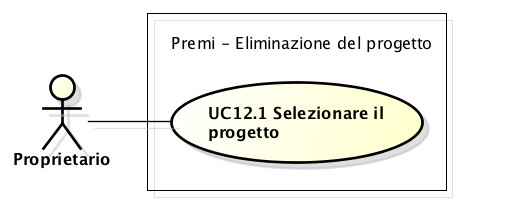
\includegraphics[scale=0.45] {img/UC12.png}
	\caption{UC12 - Eliminazione di un progetto} 
\end{figure}

\begin{itemize}
	\item \textbf{Attori:} Proprietario;
	\item \textbf{Scopo e descrizione:} L'utente vuole eliminare un progetto che ha creato in precedenza;
	\item \textbf{Precondizione:} L'utente ha già creato un progetto;
	\item \textbf{Flusso principale degli eventi:}
	\begin{enumerate}
		\item L'utente seleziona il progetto che vuole eliminare [UC12.1];
		\item L'utente conferma l'eliminazione del progetto [UC12.2].
	\end{enumerate}
	\item \textbf{Postcondizione:} Il sistema ha eliminato il progetto dal server.
\end{itemize}


\subsection{Caso d'uso UC12.1: Selezionare il progetto}
\begin{itemize}
	\item \textbf{Attori:} Proprietario;
	\item \textbf{Scopo e descrizione:} L'utente seleziona il progetto che vuole eliminare;
	\item \textbf{Precondizione:} Il sistema è in attesa che l'utente selezioni il progetto e dia il comando per eliminarlo;
	\item \textbf{Postcondizione:} Il sistema apre la finestra di dialogo per la conferma dell'eliminazione.
\end{itemize}


\subsection{Caso d'uso UC12.2: Confermare l'eliminazione}
\begin{itemize}
	\item \textbf{Attori:} Proprietario;
	\item \textbf{Scopo e descrizione:} L'utente deve confermare l'eliminazione del progetto;
	\item \textbf{Precondizione:} L'utente ha scelto il progetto e dato il comando per eliminarlo;
	\item \textbf{Postcondizione:} Il sistema ha eliminato il progetto dal server.
\end{itemize}

	% eliminazione
\newpage


\newpage
% ...

%\printglossaries

\end{document}
